\documentclass[12pt,a4paper,openright,twoside]{book}
\usepackage[utf8]{inputenc}
\usepackage{disi-thesis}
\usepackage{code-lstlistings}
\usepackage{notes}
\usepackage{shortcuts}
\usepackage{acronym}
\school{\unibo}
\programme{Corso di Laurea Magistrale in Ingegneria e Scienze Informatiche}
\title{Progettazione e sviluppo di un prototipo di simulatore ad eventi discreti reattivo}
\author{Giacomo Accursi}
\date{\today}
\subject{Laboratorio di Sistemi Software}
\supervisor{Prof. Danilo Pianini}
\cosupervisor{Dott. Gianluca Aguzzi}
\session{IV}
\academicyear{2022-2023}

% Definition of acronyms
% \acrodef{IoT}{Internet of Thing}
% \acrodef{vm}[VM]{Virtual Machine}


\mainlinespacing{1.241}

\begin{document}

\frontmatter\frontispiece

\begin{abstract}	
Max 2000 characters, strict.
\end{abstract}

\begin{dedication} % this is optional
Optional. Max a few lines.
\end{dedication}

\begin{acknowledgements} % this is optional
Optional. Max 1 page.
\end{acknowledgements}

%----------------------------------------------------------------------------------------
\tableofcontents   
\listoffigures     % (optional) comment if empty
\lstlistoflistings % (optional) comment if empty
%----------------------------------------------------------------------------------------

\mainmatter

%----------------------------------------------------------------------------------------
% Introduzione
%----------------------------------------------------------------------------------------
\chapter{Introduzione}
\label{chap:introduzione}

\section{Contesto e motivazioni}
Le simulazioni computerizzate rappresentano un pilastro fondamentale nell'ambito della ricerca scientifica, dell'ingegneria, della progettazione e dell'apprendimento, permettendo di esplorare e comprendere fenomeni complessi, simulare scenari realistici e testare ipotesi in un ambiente controllato e riproducibile. 
Paul Humphreys~\cite{Humphreys1990-HUMCS} definisce le simulazioni computerizzate come ``qualsiasi metodo implementato al computer per esplorare le proprietà di modelli matematici dove i metodi analitici non sono disponibili''. 
Le simulazioni computerizzate si riferiscono alla creazione di modelli digitali che riproducono il comportamento di sistemi reali o immaginari nel tempo. Questi modelli possono variare dalla semplice rappresentazione grafica alla simulazione di processi dinamici complessi, coinvolgendo l'interazione di molteplici variabili. 
Le simulazioni sono diventate indispensabili in diverse aree, incluse la modellazione dei sistemi naturali, economici e sociali. 

Ad alto livello, è possibile considerare una simulazione computerizzata come un metodo per lo studio di sistemi. In questa accezione più ampia del termine, ci riferisce all'intero processo, il quale include la scelta di un modello, la ricerca di un modo per implementare il modello in una forma che possa essere eseguita su un computer, il calcolo dell'output dell'algoritmo e la visualizzazione e lo studio dei dati risultati. Secondo Winsberg~\cite{Winsberg_2003}: 
\begin{quotation}
    "Gli studi di simulazione di successo fanno più che calcolare numeri. Fanno uso di una varietà di tecniche per trarre inferenze da questi numeri. Le simulazioni fanno uso creativo di tecniche di calcolo che possono essere motivate solo extra-matematicamente ed extra-teoricamente. Come tale, a differenza delle semplici computazioni che possono essere eseguite su un computer, i risultati delle simulazioni non sono automaticamente affidabili. Molto impegno e competenza vanno nel decidere quali risultati delle simulazioni sono affidabili e quali no." 
\end{quotation}
La definizione sopracitata interpreta la simulazione computerizzata come l'uso di un computer per risolvere o approssimare la soluzione delle equazioni matematiche di un modello che si intende rappresentare, sia esso reale o ipotetico. Un altro approccio è cercare di definire una simulazione come indipendente dalla nozione di simulazione al computer e poi definire ``simulazione al computer'' come una simulazione eseguita da un computer digitale programmato. Utilizzando questo approccio, una simulazione è qualsiasi sistema che si crede abbia un comportamento dinamico sufficientemente simile ad un altro sistema tale che il primo possa essere studiato per apprendere il secondo. Questo è in linea con la definizione data da Hartmann~\cite{Hartmann1996-HARTWA-2}, secondo il quale ``una simulazione imita un processo con un altro processo'', dove in questo caso il termine processo si riferisce unicamente a qualche oggetto o sistema il cui stato cambia nel tempo. Questa definizione verrà poi corretta da Huges~\cite{Hughes_1999}, il quale obiettò che la definizione di Hartmann escludeva simulazioni che imitano la struttura di un sistema piuttosto che le sue dinamiche. 
Humphreys ha revisionato~\cite{Humphreys2004-HUMEOC-2} la sua definizione di simulazione per accordarsi con le osservazioni di Hartmann e Hughes come segue: 
\begin{quotation}
    Il sistema $S$ fornisce una simulazione di base di un oggetto o processo $B$ nel caso in cui $S$ sia un dispositivo computazionale concreto che produce, attraverso un processo temporale, soluzioni a un modello computazionale che rappresenta correttamente $B$, sia dinamicamente che staticamente. Se inoltre il modello computazionale utilizzato da $S$ rappresenta correttamente la struttura del sistema reale $R$, allora $S$ fornisce una simulazione di base del sistema $R$ rispetto a $B$. 
\end{quotation}


\section{Obiettivi della tesi}
Negli ultimi vent'anni è stato compiuto un lavoro significativo sul tema dei metodi e degli approcci per ottimizzare i modelli di simulazione a eventi discreti. Allora, come oggi, una delle sfide più grandi nell'ottimizzazione delle simulazioni a eventi discreti è l'incapacità di identificare precisamente la soluzione ottimale per un determinato modello di sistema. Questo è particolarmente vero quando lo spazio delle soluzioni possibili si espande.

Negli ultimi vent'anni la velocità di calcolo è aumentata, i costi di calcolo e modellazione sono diminuiti e si sono verificati sviluppi teorici nel campo dell'ottimizzazione della simulazione. Tuttavia, la letteratura recente indica una mancanza di nuovi approcci innovativi per ottimizzare modelli di simulazione a eventi discreti su larga scala, così come un'assenza nel colmare il crescente divario tra il processo di modellazione della simulazione, ottimizzazione e miglioramento dei risultati. Molte delle ricerche e dei progressi compiuti nei primi anni '90 sono ancora citati oggi quando si discute dell'ottimizzazione della simulazione~\cite{DBLP:conf/scsc/Riley13}.
Gli approcci di ottimizzazione algoritmica si sono evoluti nel tempo man mano che la simulazione a eventi discreti è diventata più diffusa. Le tecniche di ottimizzazione coinvolgono numerose valutazioni dinamiche dello spazio delle soluzioni multidimensionale di una simulazione nella ricerca di una soluzione ottimale. Il lavoro nell'ambito dell'ottimizzazione della simulazione a eventi discreti si è concentrato principalmente sulla progettazione e valutazione di vari approcci algoritmici ed euristici nella ricerca dello spazio delle soluzioni della simulazione.

Uno degli aspetti critici, quando si parla di performance, è la gestione e l'aggiornamento delle dipendenze fra eventi duranti la simulazione. 
L'obiettivo della tesi è la progettazione e lo sviluppo di un simulatore ad eventi discreto reattivo, in grado di eliminare il grafo delle dipendenze fra eventi, utilizzato attualmente nel simulatore Alchemist, facendo uso di tecniche di programmazione reattiva. 

\section{Struttura della tesi}
Nel capitolo 2 si intende effettuare una panoramica sulle simulazioni ad eventi discreti, introducendone il funzionamento e spiegando le differenze fra simulazioni ad eventi discrete e continue. Si intende inoltre fornire un confronto fra simulazioni ad eventi discrete event-driven e time-driven. Al termine del capitolo verranno descritte le caratteristiche principali del simulatore Alchemist e le peculiarità sul suo funzionamento. 
Il capitolo 3 mira a descrivere la filosofia della programmazione reattiva, analizzandone vantaggi e criticità, astraendo però dalla loro implementazione. 
Il capitolo 4 descrive l'implementazione reattiva nel linguaggio Kotlin, parlando di come sono implementate le kotlin Coroutine e i Kotlin Flow. 
Nel capitolo 5 si potrà trovare la progettazione e l'implementazione del prototipo di simulatore. 


%----------------------------------------------------------------------------------------
% Simulazioni ad eventi discreti
%----------------------------------------------------------------------------------------
\chapter{Simulazioni ad Eventi Discreti}
\section{Panoramica sulle simulazioni ad eventi discreti}
\label{sec:panoramica-des}
Un \textbf{sistema ad eventi discreti} è un sistema a stati discreti guidato da eventi, il cui il progresso del tempo è determinato dall'occorrenza di eventi grazie ai quali il sistema evolve. Nel contesto di una simulazione ad eventi discreti, un \textbf{evento} rappresenta un cambiamento nello stato del sistema. 
Gli esempi di eventi possono includere l'arrivo di un messaggio in un sistema di comunicazione, il completamento di un processo, o qualsiasi altro avvento che influenzi il comportamento del sistema. La simulazione avanza di passi discreti, con ogni passo che corrisponde all'accadimento di un nuovo evento. 
Questo approccio è spesso utilizzato per modellare e analizzare sistemi complessi, come reti di computer, catene di approvvigionamento, code di attesa o altri scenari in cui gli eventi guidano il comportamento del sistema. 

\subsection{Terminologia e componenti}
I concetti alla base di un sistema ad eventi discreti sono i seguenti: 
\begin{itemize}
    \item \textbf{Sistema}: collezione di entità che interagiscono fra loro nel tempo per raggiungere determinati obiettivi.
    \item \textbf{Modello}: una rappresentazione astratta del sistema, spesso contenente relazioni strutturali, logiche o matematiche che descrivono il sistema stesso.
    \item \textbf{Stato del sistema}: una collezione di variabili che contengono tutte le informazioni necessarie per descrivere il sistema in ogni momento.
    \item \textbf{Entità}: un oggetto nel sistema che richiede una rappresentazione esplicita nel modello. Le entità possono essere create in fase di inizializzazione della simulazione o durante essa. 
    \item \textbf{Attributi}: sono le proprietà di una determinata entità.
    \item \textbf{Evento}: una occorrenza istantanea che cambia lo stato del sistema. 
    \item \textbf{Future Event List (FEL)}: contiene tutti gli eventi futuri ordinati cronologicamente in base al tempo di accadimento. Deve essere implementata in modo che gestisca in maniera efficiente l'aggiunta, la rimozione e la ricerca di eventi. 
    \item \textbf{Clock}: una variabile rappresentante il tempo simulato. In generale non esiste nessuna correlazione fra il tempo simulato e il tempo necessario per eseguire la simulazione. 
\end{itemize}
Una simulazione ad eventi discreti procede acquisendo una sequenza di \textit{snapshot}, i quali rappresentano l'evoluzione del sistema nel tempo. Uno snapshot ad un determinato istante $t$, include non solo lo stato del sistema al tempo $t$, ma anche la lista degli eventi futuri e lo stato di tutte le entità del sistema.

\subsection{Algoritmo Event-scheduling Time-advance}
\label{sec:time-advance-algorithm}
La dinamicità intrinseca delle simulazioni ad eventi discreti impone la necessità di gestire attentamente il flusso temporale attraverso il monitoraggio costante del clock. 
Un meccanismo fondamentale per garantire l'evoluzione accurata della simulazione, rispettando l'ordine cronologico degli eventi, è rappresentato dall'algoritmo ``\textit{event-scheduling time-advance}'', basato sull'utilizzo della future event list (FEL).

\begin{figure}
    \centering
    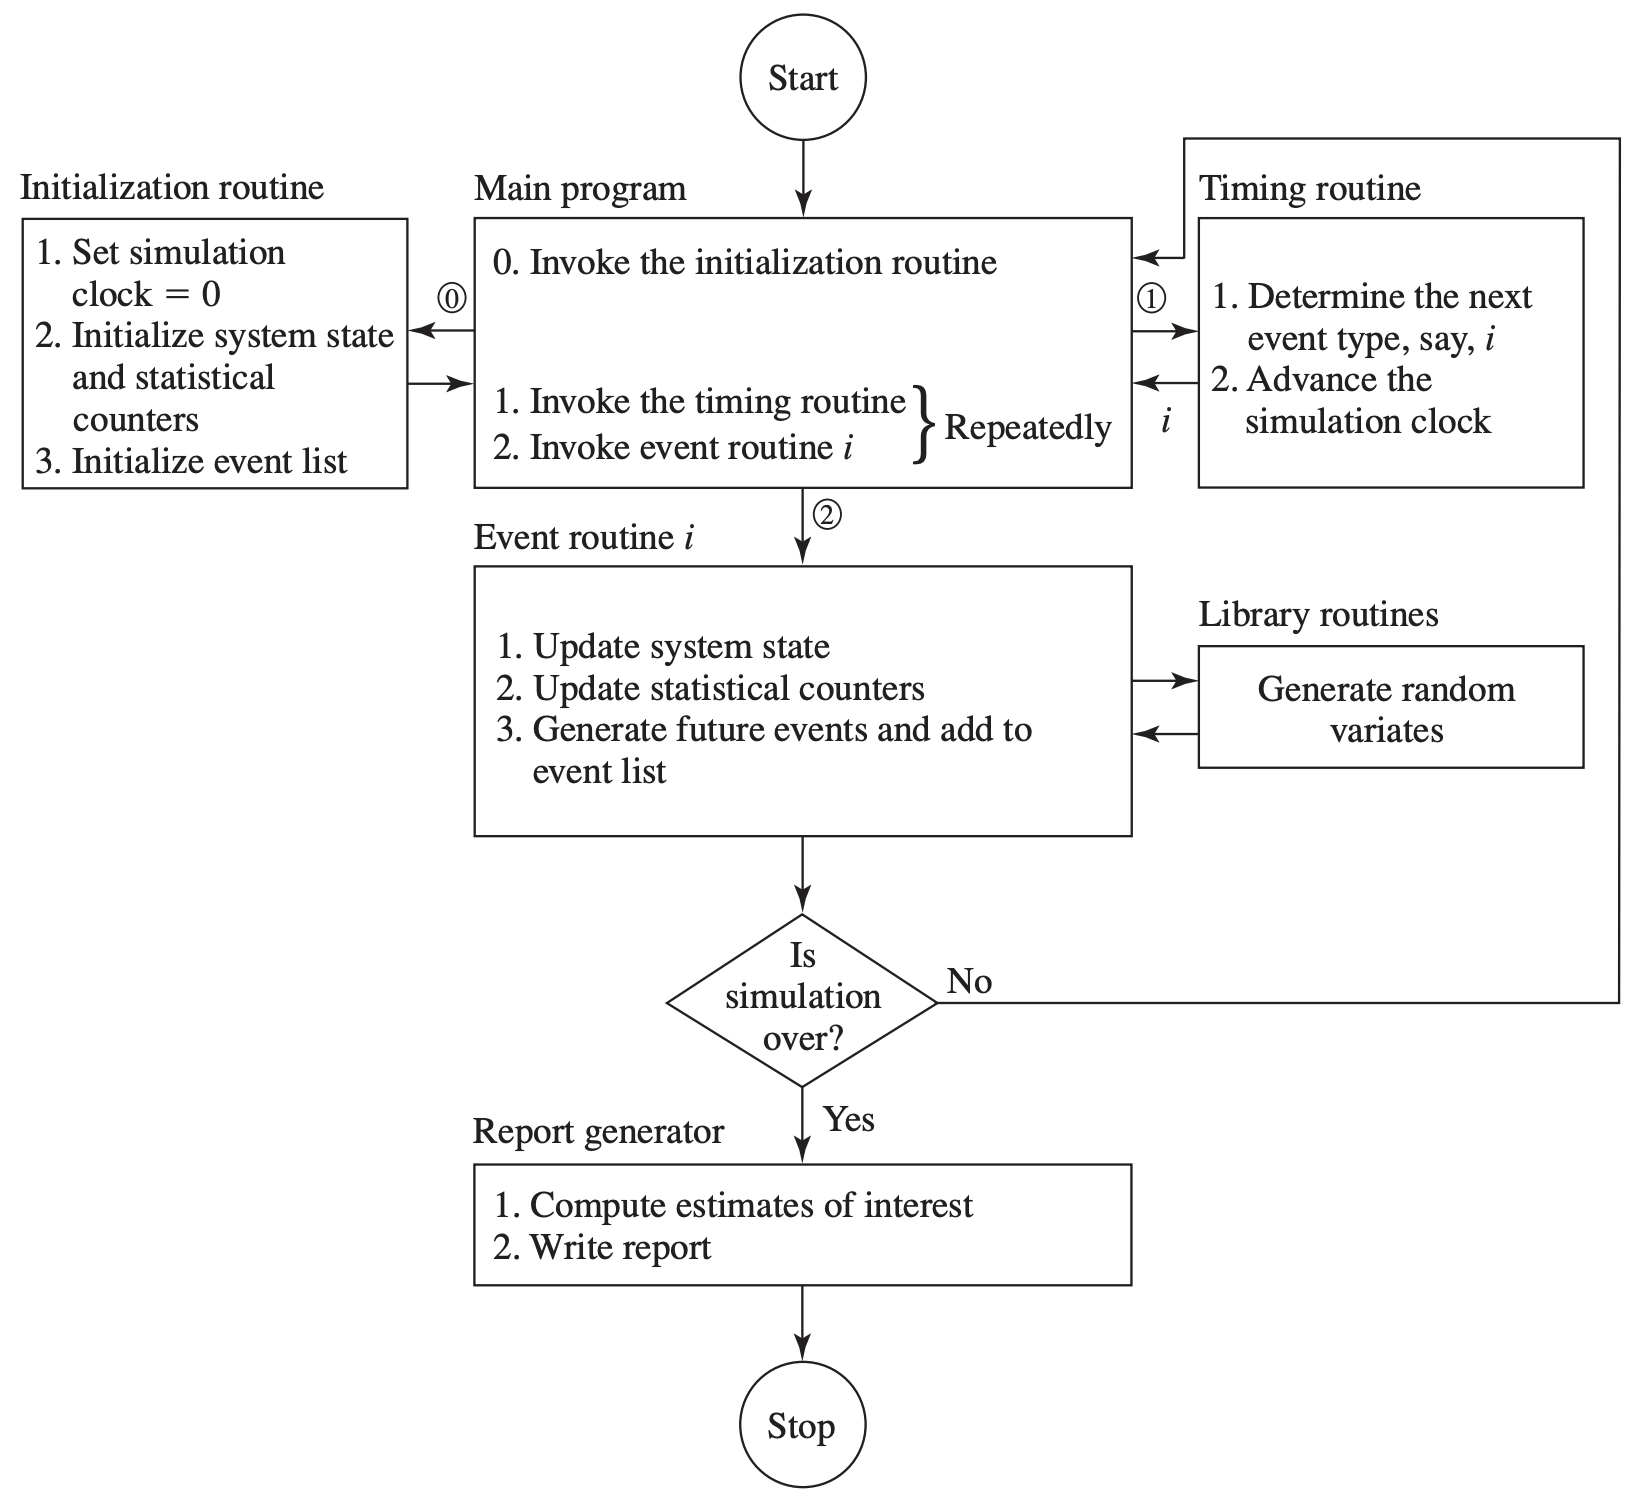
\includegraphics[width=.90\linewidth]{figures/discrete-event-simulation/time-advance-flow.png}
    \caption{Flusso di controllo dell'algoritmo event-scheduling time-advance \cite{Law15}.}
    \label{fig:next-event-flow}
\end{figure}

L'algoritmo in questione, il cui flusso di controllo è illustrato in figura~\ref{fig:next-event-flow}, è suddiviso in tre sezioni chiave: \textit{inizializzazione}, \textit{ciclo di elaborazione degli eventi} e \textit{fase di output}.
La simulazione inizia al tempo 0, quando il \textit{main program} dà avvio alla simulazione invocando la \textit{initialization routine}, nella quale il clock viene settato a 0 e le entità e le variabili di stato sono inizializzate.
Il controllo torna poi al main program, il quale invoca una \textit{timing routine} per identificare il prossimo evento da eseguire.
La lista degli eventi futuri contiene tutti gli eventi ordinati per tempo di accadimento: $FEL = [t_1, t_2, \dots t_n], t_1 \leq t_2 \leq \dots \leq t_n$. 
Il tempo $t$ è il valore corrente del clock, mentre l'evento associato al tempo $t_1$ è chiamato evento imminente, ovvero il prossimo evento che dovrà verificarsi~\cite{DBLP:books/daglib/0034857}.
Il controllo torna nuovamente al \textit{main program}, il quale invoca l'\textit{event routine} grazie al quale l'evento imminente viene eseguito effettivamente. 
L'esecuzione dell'evento imminente, seguita dalla generazione di uno snapshot correlato, comporta l'avanzamento del clock al successivo istante temporale. L'evento imminente è rimosso quindi dalla FEL ed eseguito, generando un nuovo snapshot al tempo $t_1$ basato sulla natura dell'evento e lo snapshot precedente. In questa fase nuovi eventi futuri possono essere generati e aggiunti opportunamente alla FEL.
Il processo si ripete ciclicamente fino alla conclusione della simulazione. 
Durante la fase di output vengono invece elaborate e registrate le statistiche di interesse. 

\subsubsection{Gestione Future Event List}
Una Future Event List, come anticipato, è la struttura dati che contiene l'elenco degli eventi programmati per verificarsi in futuro. Tradizionalmente l'elenco è ordinato in base al tempo di esecuzione al quale l'evento è stato schedulato, ma questo non è un requisito. 
La gestione efficiente della FEL è di fondamentale importanza, alcuni modelli di simulazione impiegano più tempo CPU nella gestione della lista piuttosto che qualsiasi altro aspetto, come per esempio la generazione di numeri casuali, l'elaborazione di eventi, l'esecuzione di operazioni aritmetiche varie ecc\dots

Nella gestione degli eventi che compongono la FEL, ci sono due operazioni critiche: l'operazione di inserimento (\textit{enqueue}) e l'operazione di cancellazione (\textit{dequeue}). Un'operazione di cancellazione viene eseguita per elaborare l'evento o perché un evento, precedentemente pianificato deve essere annullato per qualche motivo. L'inserimento e la cancellazione possono verificarsi in una posizione precisa nella lista degli eventi, oppure potrebbe essere necessario avviare una ricerca per determinare la giusta posizione. 
Importante è anche l'operazione di modifica, in cui una ricerca di evento esistente presente in lista è seguita da una modifica di qualche aspetto dell'evento stesso, come ad esempio la modifica del tempo di accadimento al quale è schedulato. 

Esistono tre criteri principali per determinare l'efficacia della struttura dati e dell'algoritmo per la gestione della FEL: 
\begin{itemize}
    \item \textbf{velocità}: la struttura dati e l'algoritmo per inserire ed eliminare un evento devono essere ottimizzate per minimizzare il tempo di esecuzione. Per ottenere tempi di esecuzione rapidi è fondamentale una ricerca degli eventi efficiente. Un algoritmo efficiente tende a valutare il  il minor numero di eventi possibile per l'inserimento o la cancellazione;
    \item  \textbf{robustezza}: è necessaria una gestione efficace degli errori per affrontare scenari imprevisti. Occorre una validazione dei dati durante l'inserimento per garantire l'integrità della struttura dati; 
    \item \textbf{adattabilità}: la FEL dovrebbe consentire la configurazione di parametri chiave per adattarsi a diverse modalità di gestione degli eventi o politiche temporali. Dovrebbe inoltre essere progettata in modo che nuove funzionalità o tipi di eventi possano essere facilmente integrati senza modificare drasticamente il codice esistente. 
\end{itemize}

\subsection{Partenza e terminazione}
Nella \Cref{sec:time-advance-algorithm} è stato descritto come la simulazione avanza durante la sua esecuzione. Tipicamente per far partire una simulazione, in fase di inizializzazione viene generato un evento specifico che viene poi inserito nella lista di eventi futuri. 
La terminazione può invece essere raggiunta tramite diversi meccanismi: 
\begin{itemize}
    \item tempo di simulazione massimo: al tempo 0 viene schedulato un evento di stop ad un tempo futuro $T_e$. In questo caso si è certi che la simulazione verrà eseguita nell'intervallo $[0, T_e]$; 
    \item eventi speciali di terminazione: il tempo di esecuzione $T_e$ è determinato dalla simulazione stessa. In genere $T_e$ dipende dal numero di occorrenze di un determinato evento. Per esempio, potrebbe essere il tempo del completamento del centesimo servizio presso un determinato centro di assistenza;  
    \item terminazione quando la FEL è vuota.
\end{itemize}
Nel secondo e nel terzo caso il tempo per eseguire la simulazione non è conosciuto a priori e può variare di simulazione in simulazione.

Le esecuzioni di una simulazione possono essere classificate in \textbf{transient} e \textbf{steady state}. La selezione del tipo di simulazione è particolarmente importante e la decisione deve essere presa in base all'output che vogliamo analizzare. Con il termine \textit{transient} ci si riferisce ad una simulazione che termina, per causa di un evento speciale o grazie ad un tempo prefissato. 
Una simulazione \textit{steady state}, al contrario, non termina mai. L'obiettivo in questo caso è studiare il comportamento a lungo termine del sistema. 

\subsection{Distribuzioni di probabilità}
Il successo di una simulazione richiede un approccio completo che va oltre la semplice creazione di un diagramma di flusso del sistema in esame, la sua traduzione in un ``programma'' per computer e la replicazione di alcune configurazioni proposte del sistema. L'uso della probabilità e della statistica è un aspetto fondamentale di uno studio di simulazione, tanto che ogni team di modellazione dovrebbe includere almeno un esperto con una solida formazione in queste tecniche~\cite{Law15}.
Per effettuare una simulazione, utilizzando input casuali come i tempi di arrivo o le dimensioni della domanda, occorre specificare le loro distribuzioni di probabilità. La scelta delle corrette distribuzioni determina in maniera importante l'accuratezza del modello. 

Nelle simulazioni ad eventi discreti è comune modellare il tempo trascorso tra gli arrivi successivi degli eventi utilizzando distribuzioni di probabilità. 
Ad esempio, nel caso di una coda di attesa in un sistema di servizio, i tempi tra gli arrivi dei clienti possono essere modellati utilizzando una \textbf{distribuzione esponenziale} o di \textbf{Poisson}. Queste distribuzioni consentono di rappresentare realisticamente il processo di arrivo degli eventi e di stimare la frequenza con cui si verificano.
I tempi di servizio potrebbero essere invece costanti o probabilistici. Se i tempi sono completamente casuali, potrebbe essere necessario dover utilizzare una \textbf{distribuzione esponenziale}. Potrebbe anche accadere che i tempi di servizio siano costanti, ma una variabilità casuale causi fluttuazioni in modo negativo o positivo. Ad esempio, il tempo impiegato da un tornio per attraversare un albero di 10 centimetri dovrebbe essere costante. Tuttavia, il materiale potrebbe presentare lievi differenze di durezza o lo strumento potrebbe usurarsi. Qualsiasi evento potrebbe causare tempi di lavorazione diversi. In questi casi la \textbf{distribuzione normale} potrebbe descrivere il tempo di servizio~\cite{DBLP:books/daglib/0034857}.
Oltre ai tempi di arrivo e di servizio, le simulazioni possono coinvolgere altre variabili casuali che influenzeranno il comportamento del sistema: i ritardi tra l'arrivo di un evento e la sua elaborazione possono essere modellati utilizzando distribuzioni di probabilità per rappresentare il tempo impiegato per completare determinate attività o processi. 

\subsection{Simulazione parallela}
La \textbf{simulazione parallela a eventi discreti} (PDES) riguarda l'esecuzione di un singolo programma di simulazione a eventi discreti su un computer sfruttando il calcolo parallelo~\cite{DBLP:journals/cacm/Fujimoto90}. Distribuendo l'esecuzione di una simulazione su più processori, si cerca di ridurre notevolmente il tempo di esecuzione del modello, fino a un fattore pari al numero di processori. Questo concetto è valido in teoria, in realtà la \textbf{legge di Amdahl} stabilisce che il miglioramento della velocità di esecuzione di un programma parallelizzabile su un sistema multi-core è limitato dalla frazione sequenziale del programma~\cite{DBLP:conf/afips/Amdahl67}. In altra parole, anche se una parte del programma può essere eseguita in modo parallelo, ci sarà sempre una parte sequenziale che non può essere parallelizzata. La legge di Amdahl può essere espressa con la seguente formula: 
$$
Speedup_{max} = \frac{1}{(1-P)+\frac{P}{N}}
$$
Dove: 
\begin{itemize}
    \item $Speedup_{max}$ è il miglioramento massimo della velocità di esecuzione ottenibile parallelizzando il programma. 
    \item $P$ è la frazione di codice che può essere parallelizzata. 
    \item $N$ è il numero di core disponibili.
\end{itemize}

Se si intende simulare un modello militare di grandi dimensioni o una rete di comunicazione contenente migliaia di nodi, il tempo di esecuzione potrebbe essere eccessivo e si potrebbe prendere in considerazione la simulazione parallela. Un altro uso della simulazione parallela potrebbe essere il processo decisionale in tempo reale. Ad esempio, in un sistema di controllo del traffico aereo, potrebbe risultare utile simulare diverse ore di traffico aereo per decidere come reindirizzarlo al meglio~\cite{DBLP:conf/wsc/Wieland98}. 

Lo sviluppo di una simulazione parallela richiede la scomposizione del modello in \textbf{processi logici} (LP). I singoli LP sono assegnati a processori diversi, ognuno dei quali si occupa di simulare la propria parte di modello. Gli LP comunicano fra loro inviandosi messaggi o eventi con data e ora.
Quando si progetta una simulazione parallela è di fondamentale importanza garantire che gli eventi del modello, indipendentemente dal loro LP, vengano elaborati nella corretta sequenza temporale, mantenendone in questo modo l'ordine causale. Se ogni LP elabora tutti i suoi eventi (generati da se stesso o da un altro LP) in ordine di tempo crescente, garantendo che gli eventi successivi siano eseguiti solo dopo quelli precedenti, e garantendo che gli eventi siano correttamente sincronizzati durante l'esecuzione in parallelo, allora l'ordine causale viene automaticamente conservato nella simulazione distribuita. Questo principio è cruciale per evitare inconsistenze e risultati non realistici.
Ogni LP può essere visto come un modello di simulazione sequenziale a eventi discreti, con le proprie variabili di stato locali, i propri eventi e il proprio clock.

Storicamente sono stati adottati due meccanismi di sincronizzazione differente: \textbf{conservativo} e \textbf{ottimistico}~\cite{DBLP:conf/wsc/Fujimoto95}.
Quando si utilizza un meccanismo conservativo l'obiettivo è evitare di violare il vincolo di causalità temporale. Ad esempio, si supponga che un particolare LP si trovi attualmente al tempo di simulazione 25 e sia pronto a elaborare il prossimo evento, che ha un tempo di 30. Il meccanismo di sincronizzazione deve assicurarsi che questo LP non riceva in seguito un evento da un altro LP con tempo di accadimento inferiore a 30. Pertanto, l'obiettivo è determinare quando è effettivamente sicuro elaborare un particolare evento. 
La sincronizzazione conservativa presenta due principali svantaggi: 
\begin{itemize}
    \item non può sfruttare appieno il parallelismo disponibile: se l'evento A influenza in qualche modo l'evento B, allora A e B devono essere eseguiti in sequenza. Se il modello è tale per cui A influisce raramente B, allora A e B potrebbero essere elaborati in modo concorrente per la maggior parte del tempo;
    \item non è robusta: una modifica apparentemente piccola del modello può inficiare le prestazioni. 
\end{itemize}
Nella sincronizzazione di tipo ottimistico, le violazioni del vincolo di causalità locale possono verificarsi, ma il meccanismo di sincronizzazione rileva le violazioni e le recupera. Anche in questo caso ogni LP simula la propria porzione di modello in avanti nel tempo, ma non aspetta di ricevere messaggi da altri processi. 
Il meccanismo \textit{time-warp}~\cite{DBLP:journals/toplas/Jefferson85} è il più noto approccio ottimistico. Se un LP riceve un messaggio che avrebbe dovuto ricevere nel suo passato (e che quindi potrebbe influenzare le sue azioni da quel momento in poi), viene effettuato un \textit{rollback} nell'LP ricevente che porta il suo clock all'ora del messaggio in arrivo.
Parte del lavoro annullato potrebbe consistere nell'invio di messaggi ad altri LP. L'invio di questi messaggi viene anch'esso annullato grazie all'invio del corrispondente anti-messaggio. L'invio di anti-messaggi può generare a sua volta rollback secondari negli LP di destinazione.
I meccanismi di sincronizzazione ottimistici possono sfruttare il parallelismo in modo migliore rispetto agli approcci conservativi, poiché non sono limitati dallo scenario peggiore. Tutta via presentano comunque alcuni svantaggi: 
\begin{itemize}
    \item comportano costi computazionali maggiori legati all'esecuzione dei rollback; 
    \item per poter effettuare i rollback lo stato di ogni LP deve essere salvato periodicamente, comportando un maggiore utilizzo di memoria.
\end{itemize}

\subsection{Cenni Storici}
La storia delle simulazioni ad eventi discreti si estende per oltre mezzo secolo, risalendo ai primi anni dell'era informatica. La necessità di modellare e comprendere il comportamento dinamico dei sistemi complessi spinse i ricercatori a sviluppare metodologie e strumenti per simulare il funzionamento di tali sistemi.
Le radici concettuali delle simulazioni ad eventi discreti possono essere rintracciate nella teoria dei processi stocastici, che ha trovato applicazioni pratiche nell'ambito dell'ingegneria, della gestione delle operazioni aziendali e della logistica. 

Nel corso degli anni '50 e '60, con l'avvento dei primi computer e l'espansione dei linguaggi di programmazione, emersero i primi tentativi di simulare sistemi complessi utilizzando modelli basati su eventi discreti. Questi primi sforzi furono spesso limitati dalle risorse computazionali disponibili e dalle limitazioni dei linguaggi di programmazione dell'epoca.

Negli anni '60 e '70, con l'avanzamento della tecnologia informatica e l'introduzione di linguaggi di programmazione più potenti, come FORTRAN e ALGOL, la simulazione ad eventi discreti divenne sempre più praticabile e diffusa. Durante questo periodo furono sviluppati i primi linguaggi di programmazione specificamente progettati per la simulazione, come SIMSCRIPT~\cite{DBLP:journals/ibmsj/DimsdaleM64} e GPSS~\cite{DBLP:journals/tssc/HollandM68}, i quali permisero ai ricercatori di modellare e analizzare sistemi complessi in modo più efficace e efficiente.

Negli anni successivi, con il continuo avanzamento della tecnologia informatica e l'introduzione di nuovi concetti e metodologie, come la simulazione ad oggetti e la simulazione basata su agenti, le simulazioni ad eventi discreti continuarono ad evolversi e a trovare sempre più applicazioni in una vasta gamma di settori. 
Molte aziende, in particolare nel settore manifatturiero, utilizzarono le simulazioni come strumento di supporto alle decisioni. 

A livello informatico il nuovo millennio è stato caratterizzato dalla potenza sempre crescente dei personal computer, dalla diminuzione del prezzo di questi ultimi e dal World Wide Web~\cite{DBLP:journals/jors/Robinson05}. Le simulazioni hanno cominciato a integrare intelligenza artificiale e machine learning per migliorare la previsione e l'ottimizzazione dei sistemi. Inoltre, la crescente disponibilità di dati in tempo reale ha portato all'adozione di approcci di simulazione ibrida che combinano modelli ad eventi discreti con dati reali per migliorare la precisione delle previsioni e delle decisioni.

\subsection{Aree di impiego}
L'adozione delle simulazioni ad eventi discreti riveste un ruolo cruciale in numerose aree di studio e applicazioni pratiche, offrendo un metodo efficace per esplorare e comprendere il comportamento dei sistemi complessi. Attraverso l'utilizzo di modelli matematici e algoritmi appropriati, le simulazioni ad eventi discreti consentono di esaminare scenari variabili, prendendo in considerazione la casualità e la complessità intrinseche dei processi reali.
In vari ambiti l'adozione di simulazioni ad eventi discreti offre numerosi vantaggi. Queste simulazioni consentono di valutare strategie, ottimizzare processi, identificare aree di miglioramento e prevedere l'andamento futuro dei sistemi analizzati. Grazie alla possibilità di eseguire esperimenti virtuali ripetibili e controllati, le simulazioni ad eventi discreti permettono agli operatori e agli studiosi di testare diverse ipotesi e strategie senza dover intervenire direttamente sui sistemi reali, riducendo così i costi e i rischi associati all'implementazione di nuove soluzioni.

\subsubsection{Sistemi di Produzione e Movimentazione dei Materiali}
I sistemi di produzione e movimentazione dei materiali rappresentano una delle applicazioni più importanti della simulazione. La simulazione è stata utilizzata con successo come supporto nella progettazione di nuove strutture produttive, magazzini e centri di distribuzione.
Le simulazioni ad eventi discreti sono utilizzate per condurre analisi sulla capacità di produzione degli impianti, considerando le specifiche delle risorse disponibili come macchinari, manodopera e materiali. Questo aiuta ad individuare sovraccarichi o sottoutilizzazioni delle risorse e a pianificare la capacità in modo efficiente. 
Oltre alla produzione, viene impiegata anche per ottimizzare la logistica, comprese le operazioni di movimentazione dei materiali, lo stoccaggio, il prelievo, il trasporto e la distribuzione. Questo comprende l'analisi della disposizione degli impianti, dei percorsi di movimentazione e delle politiche di gestione degli inventari per massimare l'efficienza complessiva e ridurre i costi operativi. 
I simulatori ad eventi discreti consentono di modellare anche i sistemi di trasporto e distribuzione dei materiali sia all'interno che all'esterno dell'impianto manifatturiero. Ciò include la pianificazione delle rotte di trasporto, l'ottimizzazione dei tempi di consegna e l'analisi dei flussi di traffico per garantire una distribuzione efficiente dei materiali.
Infine, è possibile valutare le performance attuali del sistema di produzione e movimentazione dei materiali e testare strategie di miglioramento. Questo può includere l'implementazione di nuove tecnologie, l'ottimizzazione dei processi o la riduzione degli sprechi, contribuendo a migliorare complessivamente l'efficienza e la produttività del sistema.


\subsubsection{Sistemi informatici}
La simulazione dei sistemi informatici consente di modellare e analizzare il comportamento di reti di computer, server e sistemi distribuiti. 
I simulatori possono essere utilizzati per valutare le prestazioni del sistema, misurare latenza di rete, analizzare il throughput e identificare eventuali bottleneck. Inoltre, consentono di simulare il carico di lavoro sui sistemi, aiutando a ridimensionare correttamente l'infrastruttura e a pianificare l'allocazione di risorse. 
È possibile simulare anche l'utilizzo di nuovi algoritmi o politiche di gestione delle risorse, come strategie di scheduling dei processi e politiche di gestione della memoria.
Modellare scenari di fallimento e valutare l'impatto dei guasti, valutando l'impatto di questi ultimi sulle prestazioni del sistema e sulla disponibilità dei servizi, consente di valutare la tolleranza ai guasti di sistemi informatici complessi. 
Anche la sicurezza del sistema può essere valutata, simulando scenari di minaccia e attacchi informatici, così da identificare eventuali vulnerabilità.

\subsubsection{Reti Informatiche}
La simulazione di reti informatiche consente di comprendere il comportamento dinamico delle reti e consente di valutare le prestazioni di quest'ultima, misurando parametri chiave come la \textit{latenza} e il \textit{throughput}. Questo permette di identificare e risolvere eventuali punti critici che potrebbero compromettere le prestazioni della rete. 
Studiando il traffico di rete è possibile individuare possibili congestioni di rete e adottare strategie di routing per garantire una gestione efficiente delle risorse. 
Un altro aspetto importante è la possibilità di valutare la scalabilità della rete, ovvero la sua capacità di gestire un aumento del carico di lavoro o del numero di utenti. 
Il testing di nuovi protocolli e tecnologie consente di valutare le prestazioni di nuove soluzioni prima della loro effettiva implementazione su larga scala. 
Anche in questo caso, modellando scenari di attacco e valutando la robustezza delle contromisure di sicurezza adottate, è possibile analizzare la sicurezza della rete, proteggendola da minacce esterne e garantendo la sicurezza dei dati sensibili. 

\section{Simulazioni ad eventi discreti vs continue}
Ogni modello di simulazione è la specifica di un sistema fisico (o una parte di esso) in termini di un insieme di stati ed eventi. 
Effettuare una simulazione significa imitare l'occorrenza degli eventi che evolvono nel tempo e riconoscerne gli effetti, rappresentati come stati~\cite{PDES}. 
Gli eventi futuri indotti dagli stati devono essere pianificati. Come è possibile notare in~\Cref{fig:Continuous-vs-Discrete}, in una simulazione continua i cambiamenti di stato avvengono continuamente nel tempo, mentre in una simulazione discreta il verificarsi di un evento è istantaneo e limitato a un punto selezionato nel tempo. 
Il concetto di tempo continuo modella il tempo come un continuum di punti temporali successivi. Questo implica che i dati forniti per un certo arco di tempo sono specificati come una funzione continua nel tempo. In genere si assume che questa funzione sia anche differenziabile, in modo che i cambiamenti della variabile di stato nel tempo possano essere modellate come la derivata prima della variabile stessa. Gli intervalli di tempo non svolgono un ruolo specifico come principio organizzativo. Naturalmente si può considerare qualsiasi intervallo di tempo, ma non intervalli di tempo predefiniti di lunghezza finita che strutturano l'intero modello~\cite{Ossimitz2008TheBO}. 
\begin{figure}
    \centering
    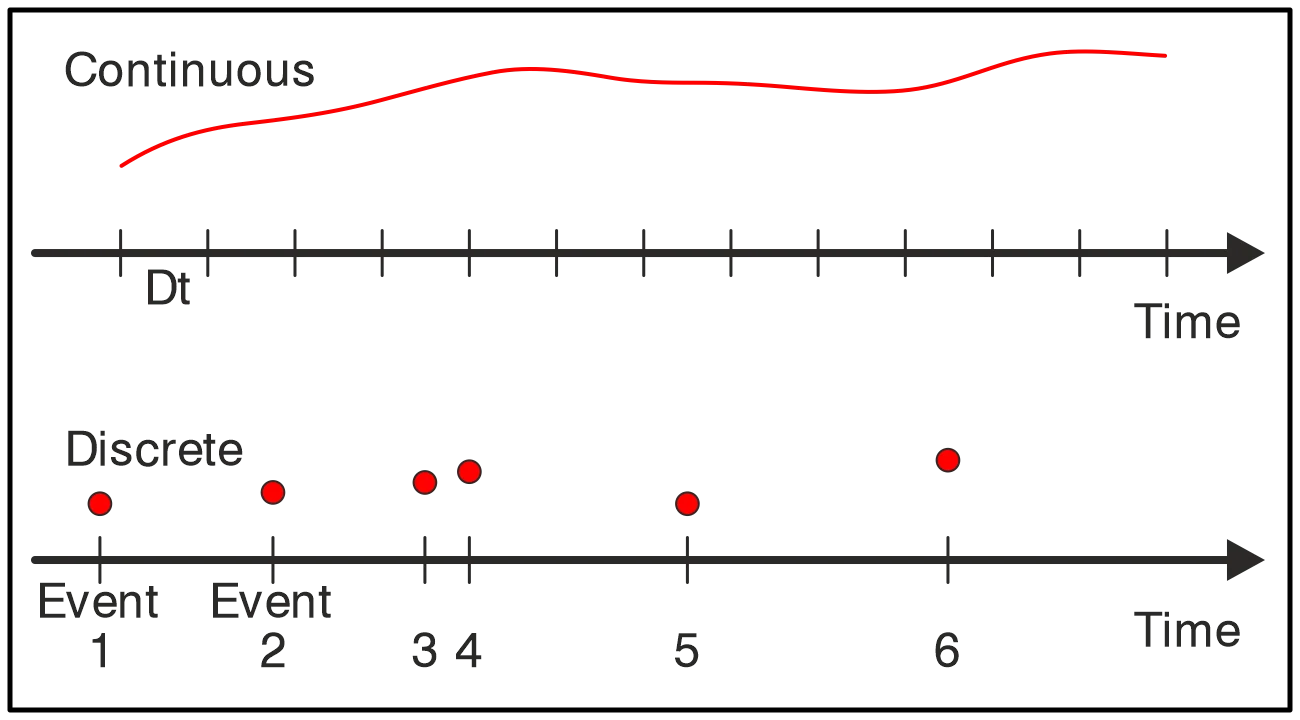
\includegraphics[width=.8\linewidth]{figures/discrete-event-simulation/Discrete-vs-Continuous-Simulation.png}
    \caption{Cambiamento di stato nel tempo in simulazioni continue vs simulazioni ad eventi discreti~\cite{Helal2008AHS}.}
    \label{fig:Continuous-vs-Discrete}
\end{figure}

Ad esempio, il livello dell'acqua in un serbatoio (la quale è una variabile di stato) può cambiare in modo continuo (ovvero con incrementi e decrementi infinitamente piccoli) e in qualsiasi punto del tempo continuo. Spesso questi modelli sono descritti da equazioni differenziali che specificano i tassi di variazione degli stati nel tempo.
Le simulazioni a tempo continuo non sono veramente continue nel senso matematico del termine, poiché per ragioni computazionali è impossibile rappresentare il tempo in modo continuo su un computer. Anche se il concetto di tempo continuo è utilizzato nella modellazione e nella simulazione, il computer deve comunque discretizzare il tempo per eseguire le simulazioni in maniera efficiente e accurata.
Ci sono diverse ragioni per cui le simulazioni a tempo continuo non possono essere veramente continue:
\begin{itemize}
    \item limitazioni computazionali: i computer hanno una quantità finita di memoria e risorse di calcolo. Per simulare un processo continuo, il tempo deve essere discretizzato in intervalli finiti. Questo porta a una rappresentazione approssimata del tempo continuo, con una risoluzione determinata dalla precisione temporale della simulazione;
    \item errori numerici: anche con un elevato numero di punti discreti nel tempo, l'approssimazione del tempo continuo introduce errori numerici. Questi errori possono accumularsi nel tempo e influenzare l'accuratezza complessiva della simulazione;
    \item algoritmi di integrazione numerica: nelle simulazioni a tempo continuo, le equazioni differenziali che descrivono il sistema devono essere risolte numericamente utilizzando algoritmi di integrazione numerica, come ad esempio il metodo di Runge-Kutta. Questi algoritmi discretizzano implicitamente il tempo per calcolare l'evoluzione del sistema nel tempo.
\end{itemize}

In generale, poiché la simulazione in tempo continuo tiene traccia dello stato del sistema in modo continuo, è più granulare e, in certe situazioni (soprattutto nelle scienze naturali), più accurata. D'altra parte, la simulazione in tempo continuo può richiedere più risorse computazionali, perché il tracciamento continuo degli stati del sistema può essere costoso.

Un'altra differenza tra le simulazioni a tempo continuo e quelle ad eventi discreti è la loro adattabilità a problemi sia continui che discreti~\cite{zgn2009DiscreteVC}. Più precisamente:
\begin{itemize}
    \item la simulazione in tempo continuo può essere utilizzata per modellare processi continui e discreti. Sebbene i processi discreti non siano continui per natura, i modelli in tempo continuo possono modellarli con successo e generare risultati validi. Ad esempio, può succedere che fenomeni come il flusso del traffico di veicoli, siano approssimati da un modello a tempo continuo considerando il traffico come un fluido. Tuttavia, un modello in tempo continuo richiederebbe più tempo e calcoli per lo stesso problema discreto. Inoltre, per alcuni sistemi discreti, l'output di un modello di simulazione in tempo continuo potrebbe non avere senso;
    \item i modelli discreti potrebbero, in teoria, essere applicati anche ai sistemi a tempo continuo. Tuttavia, un modello a eventi discreti ne fornirebbe una visione meno raffinata, a causa della sua natura.
\end{itemize}

In conclusione, è preferibile utilizzare un modello ad eventi discreti quando: 
\begin{itemize}
    \item il sistema da modellare è caratterizzato da eventi distinti che influenzano il comportamento complessivo, come code di attesa, processi di produzione, reti di computer etc\dots
    \item il sistema mostra comportamenti che possono essere modellati efficacemente attraverso una serie di eventi distinti e continui; 
    \item le risorse computazionali sono limitate o gli eventi significativi sono rari nel tempo.
\end{itemize}
Mentre è da preferire la simulazione continua quando: 
\begin{itemize}
    \item il sistema è meglio descritto da equazioni differenziali o processi che si evolvono in modo continuo nel tempo, come sistemi meccanici, flussi di traffico o processi chimici; 
    \item è necessaria una rappresentazione accurata dei cambiamenti nel tempo, specialmente quando i dettagli più sottili del comportamento sono cruciali per l'analisi; 
    \item si dispone di risorse computazionali sufficienti per gestire la complessità richiesta.
\end{itemize}

\section{Simulazioni Time-Driven vs Event-Driven}
Esistono due tipi di simulazione discreta che possono essere distinti per quanto riguarda le politiche di avanzamento nel tempo all'interno della simulazione. In una simulazione discreta \textit{time-driven} il tempo simulato avanza in passaggi temporali (o \textit{ticks}) di dimensioni constanti $\Delta$, ovvero, l'osservazione del sistema dinamico simulato è discretizzata in intervalli di tempo unitari. La scelta di $\Delta$ determina la precisione della simulazione e il tempo di simulazione trascorso: i \textit{ticks} abbastanza brevi da garantire la precisione richiesta generalmente implicano un tempo di simulazione più lungo. Intuitivamente, per strutture event-driven irregolarmente distribuite nel tempo, l'approccio \textit{time-driven} genera algoritmi di simulazione inefficienti. 

La simulazione discreta con approccio \textit{event-driven} discretizza l'osservazione del sistema simulato negli istanti in cui si verificano gli eventi. Una simulazione ad eventi discreti, quando eseguita sequenzialmente, elabora ripetutamente l'occorrenza degli eventi nel tempo simulato, mantenendo una lista di eventi ordinata per tempo che tiene traccia degli eventi temporizzati programmati per accadere in futuro, un orologio globale che indica il tempo corrente e la variabili di stato $S = (s_1, s_2, \dots, s_n)$, che definiscono lo stato attuale del sistema. Come già descritto nella \Cref{sec:panoramica-des}, un motore di simulazione guida la simulazione prendendo continuamente il primo evento dalla lista degli eventi futuri, simulando l'effetto dell'evento, cambiando le variabili di stato e eventualmente rimuovendo anche gli eventi obsoleti. Questo viene eseguito fino a quando viene raggiunto un tempo di fine predefinito, o non ci sono più eventi che devono verificarsi.

L'approccio \textit{event-driven} si concentra sulla relazione causale tra gli eventi esterni e le azioni eseguite da un sistema, ovvero sul \textbf{perché} accade qualcosa, mentre il modello \textit{time-driven} si concentra sul tempismo delle azioni, ovvero sul \textbf{quando} accade qualcosa. Nel primo caso, le azioni vengono eseguite \textbf{il prima possibile} all'arrivo degli eventi, e il tempo può essere gestito mediante segnali temporali trattati come eventi esterni asincroni. Al contrario, nel secondo caso le azioni vengono eseguite \textbf{al momento giusto} secondo un programma, e gli eventi esterni possono essere gestiti mediante meccanismi di polling~\cite{TISATO199531}.
La scelta tra i due modelli dipende dal dominio di applicazione. Nei sistemi complessi, i due modelli dovrebbero coesistere per soddisfare requisiti contrastanti. Di conseguenza, un linguaggio di programmazione dovrebbe consentire al progettista di scegliere e mescolare astrazioni per catturare nel modo più espressivo possibile i concetti chiave legati a un problema specifico o a un sotto-problema. 

\section{Simulatore Alchemist}
\label{sec:alchemist}

\textbf{Alchemist}~\cite{DBLP:journals/jos/PianiniMV13} è un simulatore ad eventi discreti open-source sviluppato all'interno dell'Università di Bologna, che permette la simulazione di scenari inerenti la computazione pervasiva ed ispirata alla natura. 
Alchemist si basa sull'algoritmo \textit{Next Reaction Method}~\cite{doi:10.1021/jp993732q}, un algoritmo di simulazione stocastica più efficiente dell'algoritmo di Gillespie~\cite{doi:10.1021/j100540a008}, su cui quest'ultimo si basa.

\subsection{Modello del dominio}
Il dominio di Alchemist, rappresentato in~\Cref{fig:alchemist-model}, è descritto dalle seguenti entità: 
\begin{itemize}
    \item \textbf{Molecola}: il nome dei data item. Se Alchemist fosse un linguaggio imperativo, una molecola potrebbe rappresentare il nome di una variabile. 
    \item \textbf{Concentrazione}: il valore associato a una particolare molecola. In un linguaggio imperativo la concentrazione sarebbe il valore associato alla variabile. 
    \item \textbf{Nodo}: un contenitore di molecole e reazioni, che vivono all'interno di un environment. 
    \item \textbf{Environment}: è l'astrazione di Alchemist per lo spazio. È un contenitore di nodi con le seguenti funzionalità: 
    \begin{itemize}
        \item è capace di dirci dov'è un nodo nello spazio;
        \item è capace di dirci la distanza fra due nodi;
        \item opzionalmente ha il supporto per rimuovere i nodi.
    \end{itemize}
    \item \textbf{Regola di collegamento}: una funzione dello stato corrente dell'environment che associa ad ogni nodo un vicinato. 
    \item \textbf{Vicinato}: un'entità composta da un nodo e un insieme di nodi vicini. Il concetto di vicino deve essere il più generale e flessibile possibile: dal concetto fisico di agenti all'interno di un raggio, al concetto sociale di due agenti collegati da una relazione sociale di qualche tipo. 
    \item \textbf{Reazione}: il concetto di reazione è più elaborato di quello usato nella chimica: nei modelli classici, una reazione elenca un certo numero di molecole reagenti che, combinate, producono un insieme di molecole prodotto. In Alchemist una reazione è un evento capace di cambiare lo stato dell'environment. Ogni nodo ha un possibile insieme (anche vuoto) di reazioni. Ogni reazione è definita da una lista (anche vuota) di condizioni, una o più azioni ad essa associate e una distribuzione temporale. La frequenza con la quale accade dipende da:
    \begin{itemize}
        \item un parametro a tasso statico; 
        \item il valore di ciascuna condizione; 
        \item una distribuzione temporale;
        \item un'equazione che a partire dal tasso statico e dai valori delle condizioni restituisce un tasso istantaneo.
    \end{itemize}
    Il suo funzionamento può essere osservato in~\Cref{fig:alchemist-reaction}
    \item \textbf{Condizione}: una funzione che prende come input l'environment corrente e restituisce in output un booleano. Per poter essere innescata, una reazione necessita che tutte le condizioni ad essa associate siano soddisfatte. Le condizioni sono tipicamente espresse come un elenco di annotazioni che devono essere disponibili in una località per l'esecuzione della reazione, ma possono anche includere considerazioni sulla forma del vicinato.
    \item \textbf{Azione}: modella i cambiamenti dell'environment. Le azioni possono essere la trasformazione, la rimozione o la produzione di annotazioni, lo spostamento di agenti, la duplicazione di essi e così via.
\end{itemize}

\begin{figure}
    \centering
    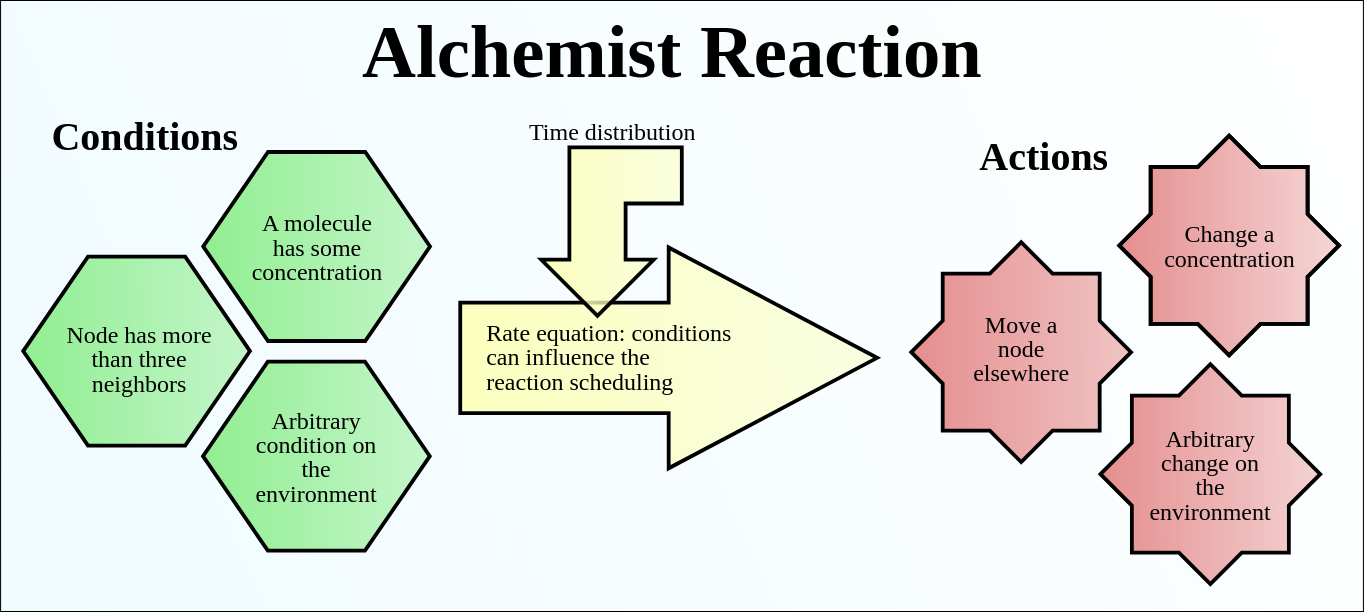
\includegraphics[width=.85\linewidth]{figures/discrete-event-simulation/alchemist-reaction.png}
    \caption{Rappresentazione grafica del funzionamento di una reazione.}
    \label{fig:alchemist-reaction}
\end{figure}

\begin{figure}
    \centering
    \includegraphics[width=.85\linewidth]{figures/discrete-event-simulation/alchemist-model.png}
    \caption{Meta-modello alla base di Alchemist.}
    \label{fig:alchemist-model}
\end{figure}

Una delle caratteristiche principali del simulatore è la sua generalità. Essa viene raggiunta attraverso l'uso delle \textbf{incarnazioni}, ovvero le istanze concrete del meta-modello in cui ogni entità viene mappata ad un corrispettivo concetto dell'universo di interesse. 
Un'incarnazione di Alchemist include una definizione del tipo di concentrazione ed eventualmente un insieme di condizioni specifiche, azioni e (raramente) ambienti e reazioni che operano su tali tipi. 
Incarnazioni diverse possono modellare universi completamente diversi. Per esempio, come nel caso di \textbf{Biochemistry}, se la concentrazione viene definita come un numero intero positivo e vengono fornite azioni e condizioni adeguate, Alchemist diventa un simulatore stocastico di chimica con compartimenti interconnessi e mobili.
\textbf{SAPERE} è l'incarnazione più vecchia. In questa incarnazione le concentrazioni sono un insieme di tuple Linda-Like. È stata utilizzata per simulare evacuazione di folle, l'adattamento anticipato e l'esplorazione di risorse.  
Nel caso di \textbf{Protelis}, la concentrazione è definita come Java Object. In questa incarnazione i nodi eseguono specifiche scritte nel linguaggio Protelis~\cite{DBLP:conf/sac/PianiniVB15}. \textbf{Scafi} è dedicata alla programmazione aggregata ed è basata sul framework Scafi~\cite{DBLP:journals/softx/CasadeiVAP22}.

\subsection{Funzionalità e utilizzo del simulatore}
Per configurare una simulazione in Alchemist, è necessario fornire un file in formato YAML\footnote{https://yaml.org/}. Nel file di configurazione occorre specificare quali classi e parametri utilizzare. Le entità vengono identificate tramite chiavi. Al livello zero è possibile trovare: 
\begin{itemize}
    \item \textbf{incarnation}: è l'unica chiave obbligatoria. Serve a specificare quale incarnazione si intende utilizzare; 
    \item \textbf{seed}: specifica il seme da utilizzare per generazione di numeri casuali. Questo serve a garantire la riproducibilità degli esperimenti scientifici. È essenziale, a fini di debug, riuscire a garantire simulazioni sempre uguali partendo dalla stessa configurazione nel file YAML;
    \item \textbf{variables}: i valori che si intendono riutilizzare all'interno del file di configurazione;
    \item \textbf{environment}: la tipologia di ambiente dentro al quale si intende eseguire la simulazione;
    \item \textbf{network-model}: permette di decidere come devono essere collegati fra loro i nodi;
    \item \textbf{export}: permette la configurazione e la scelta dei dati della simulazione che si intende esportare; 
    \item \textbf{deployment}: permette di definire quali sono i nodi del sistema e dove si trovano. 
\end{itemize}
Il simulatore può essere eseguito in due modalità: \textit{interattiva} o \textit{batch}. Nella prima viene eseguita una sola simulazione per volta mentre nella seconda vengono eseguite molteplici simulazioni che dipendono dai valori delle variabili impostati dall'utente. Impostando multipli valori per ciascuna variabile, il simulatore eseguirà una simulazione per ogni possibile combinazione di esse. 

Alchemist supporta il caricamento delle planimetrie e delle mappe geografiche. Il caricamento di una planimetria avviene a partire da un'immagine, convertendo i pixel adiacenti del colore specificato in ostacoli. Il supporto agli standard GPX e GPS rende invece possibile il caricamento di mappe. 
\subsection{Architettura}
Il framework, la cui architettura ad alto livello è osservabile in~\Cref{fig:alchemist-architecture}, è stato progettato per essere modulare ed estendibile. L'engine può essere re-implementato senza toccare niente del modello e il modello può essere esteso senza necessità di modificare l'engine. 

\begin{figure}
    \centering
    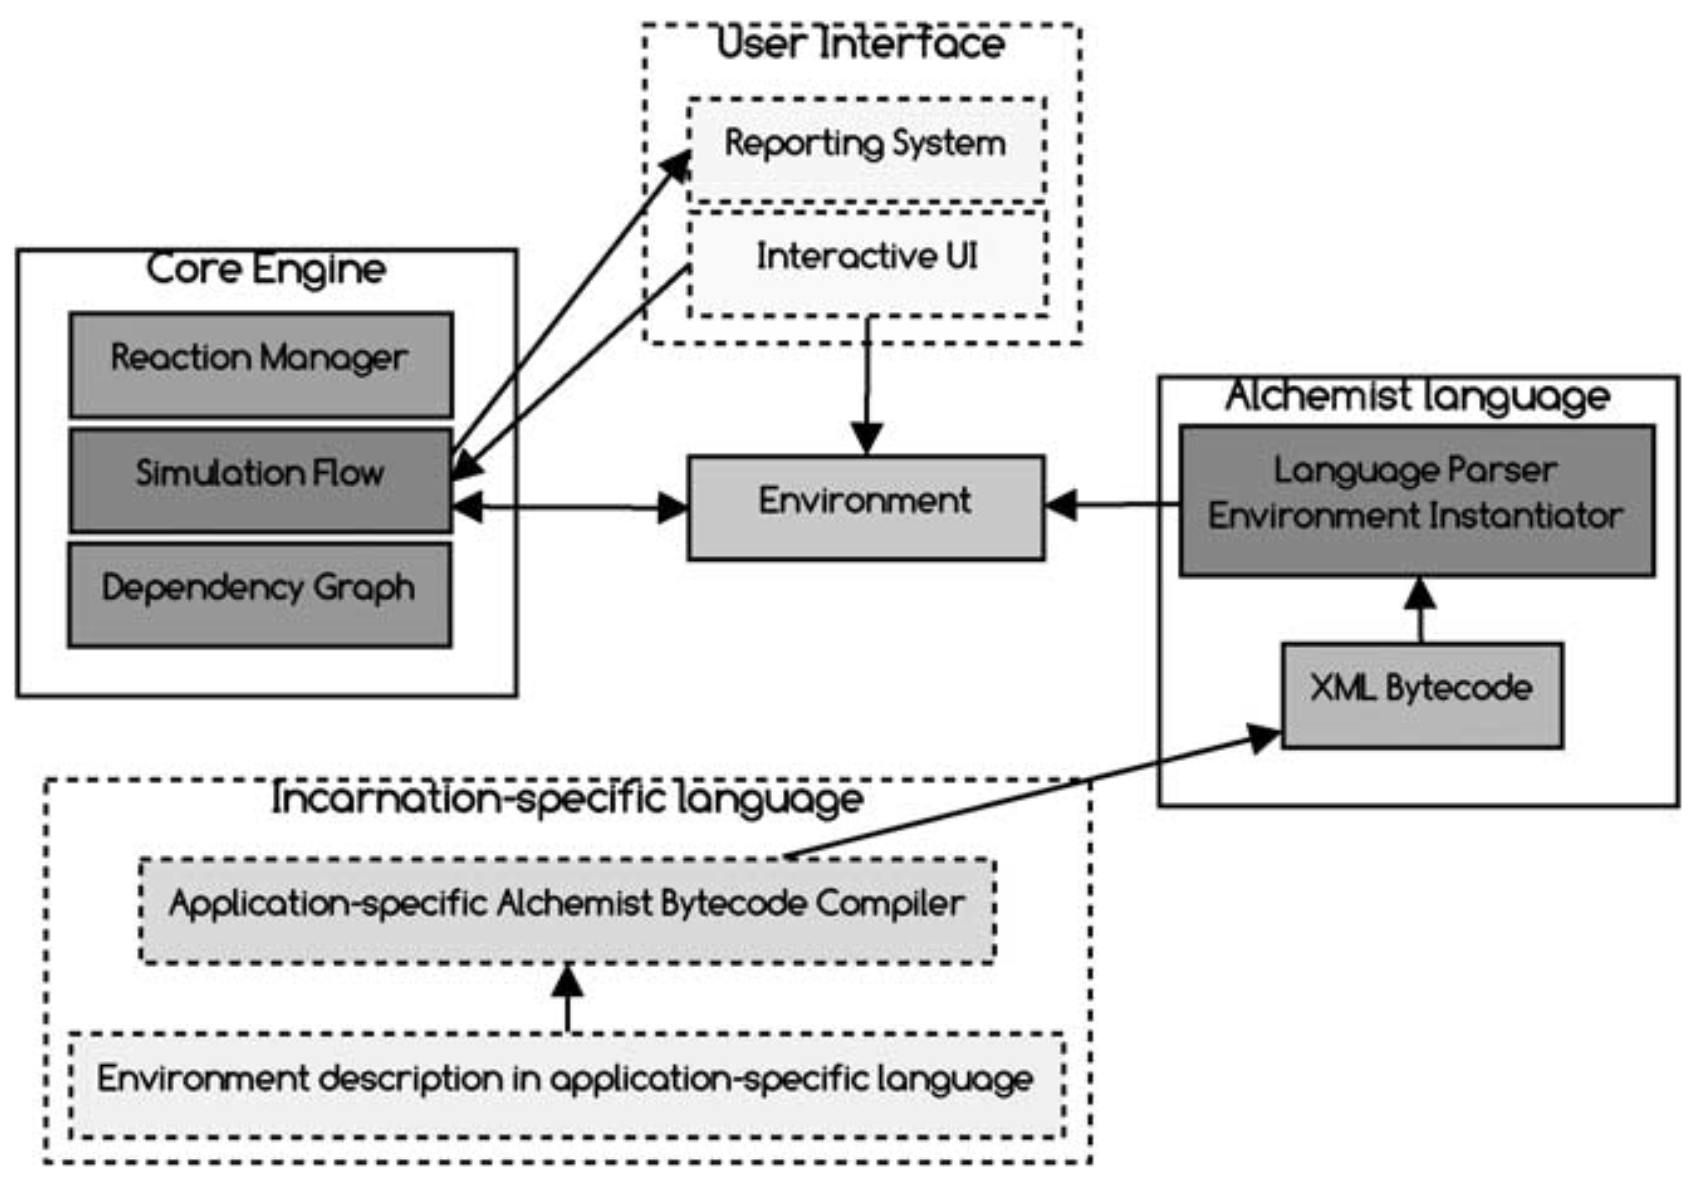
\includegraphics[width=.85\linewidth]{figures/discrete-event-simulation/alchemist-architecture.png}
    \caption{Architettura di Alchemist. Gli elementi disegnati con linee continue indicano i componenti comuni a tutti gli scenari, quelli con linee tratteggiate rappresentano componenti che devono essere sviluppati da una specifica incarnazione~\cite{DBLP:journals/jos/PianiniMV13}.}
    \label{fig:alchemist-architecture}
\end{figure}

\subsubsection{Engine}
Di seguito si intende descrivere brevemente il funzionamento dell'algoritmo \textit{Next Reaction Method}, utilizzato da Alchemist per selezionare il prossimo evento da eseguire e il \textit{Dynamic Dependency Graph}, utilizzato per gestire le dipendenze fra le reazioni presenti all'interno dei nodi. 
\paragraph{Next Reaction Method}
\label{sec:next-reaction-method}
Come anticipato, Alchemist si basa sull'algoritmo di simulazione stocastica \textit{Next Reaction Method}. Ad ogni step della simulazione è in grado di selezionare la prossima reazione da eseguire in tempo costante. L'algoritmo richiede tempo logaritmico per aggiornare la struttura dati interna. L'algoritmo non sceglie la prossima reazione da eseguire valutando la sua velocità, ma generando un tempo putativo e ordinando le reazioni per decidere quale sia la prossima da eseguire. L'algoritmo originale è stato modificato per consentire di aggiungere, rimuovere o spostare le reazioni in modo dinamico. 
Le reazioni vengono memorizzate in una \textit{Dynamic Indexed Priority Queue}. Quest'ultima è un albero binario di reazioni la cui proprietà principale è che ogni nodo memorizza una reazione il cui tempo di accadimento presunto è inferiore a quello di ciascuno dei suoi figli. Ciò significa che la prossima reazione da eseguire sarà sempre quella nella radice dell'albero e ci si potrà quindi accedere in tempo costante. 
Un'altra proprietà importante della \textit{priority queue} è che in assenza dell'aggiunta di nuovi nodi all'albero, lo swap fra due nodi non ne modifica il bilanciamento. 
In Alchemist i nodi vengono aggiunti e quindi non si riesce a sfruttare direttamente questa proprietà. L'idea è quindi di tenere traccia, per ogni nodo, del numero di discendenti per ogni ramo, avendo così la possibilità di mantenere bilanciato l'albero a seguito dell'aggiunta di nodi. 

\paragraph{Dynamic Dependency Graph}
Consiste in un grafo diretto, nel quale i nodi sono le reazioni e gli archi connettono una reazione $r$ a tutti i nodi che dipendono da essa, ovvero quelli il cui tempo di attivazione deve essere aggiornato a seguito dell'esecuzione di $r$. 
Mantenere il grafo delle dipendenze aggiornato durante la simulazione è uno dei task più critici. Dato che si vuole supportare nativamente l'interazione fra nodi, che diventano dipendenze fra le reazioni che avvengono in questi nodi, sono definiti tre \textit{contesti} (chiamati anche \textit{scopes}): 
\begin{itemize}
    \item \textbf{locale}: la reazione influenza solo il nodo in cui avviene; 
    \item \textbf{vicinato}: la reazione influenza il suo nodo e tutto il vicinato; 
    \item \textbf{globale}: la reazione influenza tutte le altre reazioni. 
\end{itemize}

Ogni reazione ha un \textbf{contesto di input}, ovvero il contesto più piccolo in cui una reazione può leggere informazioni, e un \textbf{contesto di output}, ovvero il contesto più piccolo nel quale una reazione può effettuare modifiche. 
La scelta del contesto giusto è cruciale: se è troppo ristretto la simulazione sarà invalida, se viene scelto troppo grande, questo impatterà pesantemente sulle performance. 

L'aggiunta di una reazione implica la verifica delle sue dipendenze con tutte le reazioni del sistema. Se esiste, questa dipendenza viene aggiunta al grafo delle dipendenze. La rimozione di una reazione richiede l'eliminazione di tutte le dipendenze in cui quest'ultima è coinvolta, sia come influenzante che come influenzata. 
In caso di cambiamento della topologia del sistema è necessario un ulteriore controllo delle dipendenze tra le reazioni appartenenti ai nodi che hanno subito un cambiamento del proprio vicinato. Occorre eseguire una scansione in questi nodi, calcolando le nuove dipendenze con le reazioni appartenenti ai nuovi vicini e cancellando quelle con i nodi che non appartengono più al vicinato.

%----------------------------------------------------------------------------------------
% Programmazione reattiva
%----------------------------------------------------------------------------------------
\chapter{Programmazione reattiva}
\section{Concetti chiave}
L'uso del termine \textbf{programmazione reattiva} nella letteratura scientifica risale alla metà degli anni `60. Una definizione rilevante è stata data da G. Berry nel 1991~\cite{DBLP:journals/pieee/BenvenisteB91}. Berry descrive i \textit{programmi reattivi} in relazione alla loro controparte duale, i \textit{programmi interattivi}: 
\begin{quotation}
    "I programmi interattivi interagiscono alla propria velocità con gli utenti o con altri programmi; dal punto di vista dell'utente, un sistema time-sharing è interattivo. Anche i programmi reattivi mantengono una continua interazione con l'ambiente, ma a una velocità che è determinata dall'ambiente e non dal programma stesso"
\end{quotation}
I programmi interattivi concretizzano l'idea di un modello di calcolo ``\textit{pull-based}'', in cui il programma - in questo caso il consumatore - ha il controllo sulla velocità con cui i dai vengono richiesti e gestiti. 
Un esempio perfetto di programma interattivo è una struttura di flusso di controllo come un \textit{ciclo for} che itera su un insieme di dati: il programma ha il controllo della velocità con cui i dati vengono recuperati dalla collezione e richiederà l'elemento successivo solo aver terminato la gestione di quello attuale. 

I programmi reattivi, al contrario, incarnano l'idea di un modello di calcolo ``\textit{push based}'', in cui la velocità con la quale il programma interagisce con l'ambiente è determinata dall'ambiente stesso piuttosto che dal programma. In altre parole, ora è il produttore dei dati a determinare la velocità con cui si verificheranno gli eventi, mentre il ruolo del programma si riduce a quello di un osservatore silenzioso che reagisce alla ricezione di essi. Esempi standard di tali sistemi sono le applicazioni con \textit{graphical user interface} (GUI) che si occupano di vari eventi originati dall'input dell'utente, come per esempio il click del mouse. Queste applicazioni sono difficili da programmare con i tradizionali approcci di programmazione sequenziale, perché è impossibile prevedere o controllare l'ordine di arrivo degli eventi esterni. Inoltre quando si verifica un cambiamento di stato in un calcolo o in un dato, il programmatore deve aggiornare tutti gli altri che dipendono da esso. Questa gestione manuale dei cambiamenti di stato e delle dipendenze dei dati è complessa e soggetta ad errori.

Utilizzando soluzioni di programmazione tradizionali, le applicazioni interattive sono tipicamente costruite attorno alla nozione di \textit{callback} asincrone. 
Coordinare le callback può essere un compito arduo, poiché numerosi frammenti di codice isolati possono manipolare gli stessi dati e il loro ordine di esecuzione non è prevedibile. Inoltre, le callback solitamente non hanno un valore di ritorno, quindi sono richiesti side-effect per modificare lo stato dell'applicazione~\cite{DBLP:phd/us/Cooper08}. 

Il paradigma della programmazione reattiva è stato recentemente proposto come soluzione adatta allo sviluppo di applicazioni \textit{event-driven}. La programmazione reattiva affronta i problemi posti dalla applicazioni \textit{event-driven} fornendo astrazioni per esprimere i programmi come reazioni a eventi esterni e facendo in modo che il linguaggio gestisca automaticamente il flusso del tempo e le dipendenze di dati e calcoli. Ciò porta un vantaggio per i programmatori, i quali non devono preoccuparsi dell'ordine degli eventi e delle dipendenze di calcolo. I linguaggi di programmazione reattivi astraggono dalla gestione del tempo, proprio come i \textit{garbage collector} astraggono dalla gestione della memoria. 

\section{Propagazione del cambiamento}
La programmazione reattiva è un paradigma che si basa sulla nozione di valori variabili e continui nel tempo e sulla \textbf{propagazione del cambiamento}. 
In questo paradigma i cambiamenti di stato vengono automaticamente ed efficientemente propagati attraverso la rete di computazioni dipendenti dal modello di esecuzione sottostante.

Si consideri un semplice esempio di calcolo della somma di due variabili.
\begin{quotation}\noindent
    \texttt{var1 = 1} \newline
    \texttt{var2 = 2} \newline
    \texttt{var3 = var1 + var2}
\end{quotation}
Nella programmazione sequenziale imperativa convenzionale il valore della variabile \texttt{var3} conterrà sempre il valore 3, ovvero la somma dei valori iniziali delle variabili \texttt{var1} e \texttt{var2}.
Nella programmazione reattiva il valore di \texttt{var3} è sempre aggiornato perché viene ricalcolato ogni volta che il valore di \texttt{var1} o \texttt{var2} cambia.
Questa è la nozione chiave della programmazione reattiva. I valori cambiano nel tempo e tutti i calcoli dipendenti vengono automaticamente rieseguiti. Nella terminologia della programmazione reattiva la variabile \texttt{var3} è detta dipendente dalle variabili \texttt{var1} e \texttt{var2}. La dipendenza in questione può essere osservata in~\Cref{fig:rp-dependency}.

La logica della propagazione del cambiamento può essere implementata per mezzo di un grafo i cui nodi rappresentano i valori da tenere aggiornati e gli archi rappresentano le relazioni di dipendenza che coinvolgono i nodi. Utilizzando questo tipo di architettura si viene quindi a creare una rete di dipendenze computazioni ed il cambiamento di un nodo (quindi di un valore) scatena una reazione che implica l'attraversamento degli eventuali archi ad esso collegati e il conseguente aggiornamento di tutti i nodi raggiunti. 

\begin{figure}
    \centering
    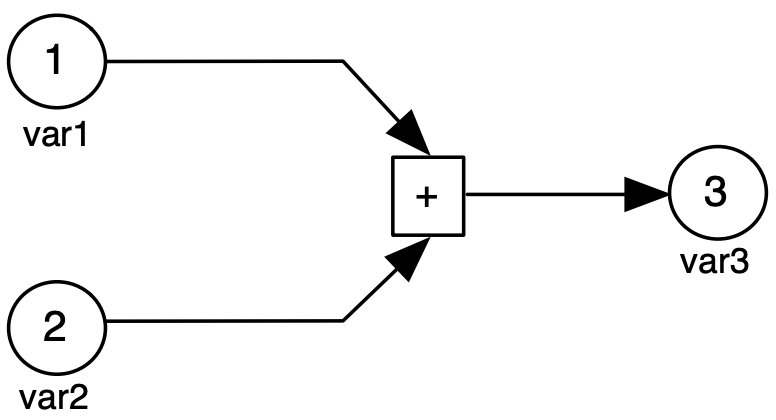
\includegraphics[width=.65\linewidth]{figures/reactive-programming/RP-dependency.png}
    \caption{Rappresentazione grafica della dipendenza fra espressioni nella programmazione reattiva \cite{DBLP:journals/csur/BainomugishaCCMM13}.}
    \label{fig:rp-dependency}
\end{figure}

\subsection{Strategie di propagazione}
Esistono diverse strategie adottabili per la propagazione del cambiamento nella programmazione reattiva, di seguito verranno descritte le principali:
\begin{itemize}
    \item \textbf{complete propagation}: ogni nodo, durante la propagazione, invia il suo stato attuale completo ai nodi dipendenti. In questo caso tutto lo stato precedente del nodo viene perso durante l'aggiornamento del nuovo stato. Questa strategia non è adatta nei casi in cui il grafo delle dipendenze sia particolarmente complesso o nel caso in cui gli stati necessitino di grandi quantità di dati per essere descritti, a causa del suo alto carico computazionale;
    \item \textbf{delta propagation}: al momento della propagazione i nodi interessati inviano solo una porzione (un \textit{delta}) del loro stato ai nodi dipendenti, cioè solo le frazioni di informazione che sono state effettivamente coinvolte da modifiche. Questo approccio tende a minimizzare la quantità di dati da trasportare lungo la catena di dipendenze durante la propagazione dei cambiamenti, dunque risulta efficiente anche nei casi in cui si ha un grafo delle dipendenze complesso e una grande quantità di dati per la rappresentazione degli stati; 
    \item \textbf{batch propagation}: prevede un ritardo nella propagazione dei cambiamenti, cioè la rappresentazione ritardata nel tempo. Consente l'ottimizzazione di quelle situazioni in cui abbiamo più cambiamenti vicini nel tempo che si annullano a vicenda e fanno sì che si ritorni allo stato di partenza. Nel caso in cui due o più cambiamenti vicini nel tempo generino un'effettiva mutazione di stato nel grafo viene propagato solo l'ultimo cambiamento, scartando i precedenti, ormai obsoleti. Questa strategia tende a minimizzare il numero di propagazioni e di conseguenza il carico computazionale complessivo. 
    Tuttavia, occorre adottare un tempo di ritardo corretto al fine di ridurre il carico computazionale, ma al tempo stesso garantire una buona reattività; 
    \item \textbf{invalidity notification propagation}: potrebbe essere definita come una ``sotto-strategia'' piuttosto che una vera e propria strategia implementativa. Consiste nella richiesta di aggiornamento da parte di un nodo che riscontra di possedere uno stato non valido, oppure che riceve un messaggio di propagazione non valido. In questo caso il nodo interessato scarta l'anomalia e richiede ai nodi da cui dipende un nuovo aggiornamento. 
\end{itemize}

\section{Modelli di valutazione}
Nella programmazione reattiva, per \textbf{modello di valutazione} (\textit{evaluation model}) si intende la dinamica direzionale che viene adottata per gestire la propagazione dei cambiamenti nel grafo delle dipendenze computazionali. 
Il modello viene applicato a livello di linguaggio, rimanendo quindi trasparente all'utilizzatore finale. 
I modelli presenti in letteratura sono due, ai quali si aggiunge un terzo, ibrido fra i primi due: 
\begin{itemize}
    \item \textbf{push-based}: nel modello \textit{push-based} la reazione inizia quando un nodo produttore cambia stato, aggiornandosi. Il nodo in questione ``spinge'' l'informazione attraverso i nodi consumatori, ovvero i nodi dipendenti. Questo approccio, guidato dalla disponibilità di nuove informazioni, ha il vantaggio di rendere il sistema altamente reattivo, in quanto le reazioni vengono provocate e propagate immediatamente dopo la disponibilità di nuovi dati. Questo approccio comporta, d'altra parte, a computazioni superflue e un alto carico di calcolo, a causa delle elaborazioni necessarie ad ogni cambiamento di stato del produttore. 
    \item \textbf{pull-based}: nel modello \textit{pull-based} sono i nodi consumatori a richiedere i nuovi valori nel momento in cui ne hanno bisogno. L'approccio in questo caso è guidato dalla domanda di nuovi dati da parte dei nodi dipendenti. Questo porta ad un sistema più flessibile, ma introduce latenze fra il momento in cui un cambiamento si verifica e il momento in cui avviene la reazione. 
    \item \textbf{hybrid push-pull}: il modello ibrido combina i due modelli \textit{push} e \textit{pull}, cercando di trarre i vantaggi di entrambe le soluzioni. Il modello \textit{push-based} funziona bene quando è richiesta una reazione istantanea al cambiamento, mentre il modello \textit{pull-based} porta a prestazioni migliori quando nel sistema si presentano continui cambiamenti di valori nel tempo. Questo approccio riesce quindi a trarre i benefici del modello \textit{push-based} (efficienza e latenza bassa) e del modello \textit{pull-based} (flessibilità nella richiesta dei valori)~\cite{DBLP:conf/haskell/Elliott09}.  
\end{itemize}


\section{Glitch}
\label{sec:glitch}
In programmazione reattiva un \textbf{glitch} indica un malfunzionamento dovuto ad una inconsistenza dei dati presenti nel grafo delle dipendenze computazionali. La prevenzione dei glitch è un'altra proprietà che deve essere presa in considerazione in un linguaggio reattivo~\cite{DBLP:journals/csur/BainomugishaCCMM13}.
Un glitch può essere provocato da una anomalia durante la propagazione di un cambiamento, oppure dal calcolo di un'espressione presente in un nodo prima della valutazione di tutte le sue dipendenze. Il risultato è una situazione nella quale un nodo esegue la propria computazione utilizzando alcuni dati aggiornati ed altri ormai obsoleti, provocando quasi certamente errori di calcolo ed inconsistenze. 
Si consideri il seguente esempio: 
\begin{quotation}\noindent
    \texttt{var1 = 1}\newline
    \texttt{var2 = var1 * 1}\newline
    \texttt{var3 = var1 + var2}
\end{quotation} 
In questo esempio, il valore della variabile \texttt{var2} dovrebbe essere sempre lo stesso di \texttt{var1}, e il valore di \texttt{var3} dovrebbe invece essere il doppio di \texttt{var1}. Inizialmente quando il valore di \texttt{var1} è 1, il valore di \texttt{var2} è 1, e quello di \texttt{var3} è 2. Se il valore di \texttt{var1} cambia, per esempio diventa 2, ci si aspetta che il valore di \texttt{var2} diventi 2 e di conseguenza quello di \texttt{var3} diventi 4. Tuttavia, in una implementazione reattiva non corretta, il cambiamento del valore di \texttt{var1} potrebbe causare il ricalcolo di \texttt{var1 + var2} prima di \texttt{var1 * 1} . In questo caso il valore di \texttt{var3} sarebbe momentaneamente 3, ovvero un valore non corretto.
Prima o poi l'espressione \texttt{var1 * 1} sarà computata, in quel momento il valore di \texttt{var2} diventerà 2 e quello di \texttt{var3} sarà ricalcolato, riflettendo il valore corretto 4. Il comportamento appena descritto è osservabile in~\Cref{fig:rp-glitch}.

\begin{figure}
    \centering
    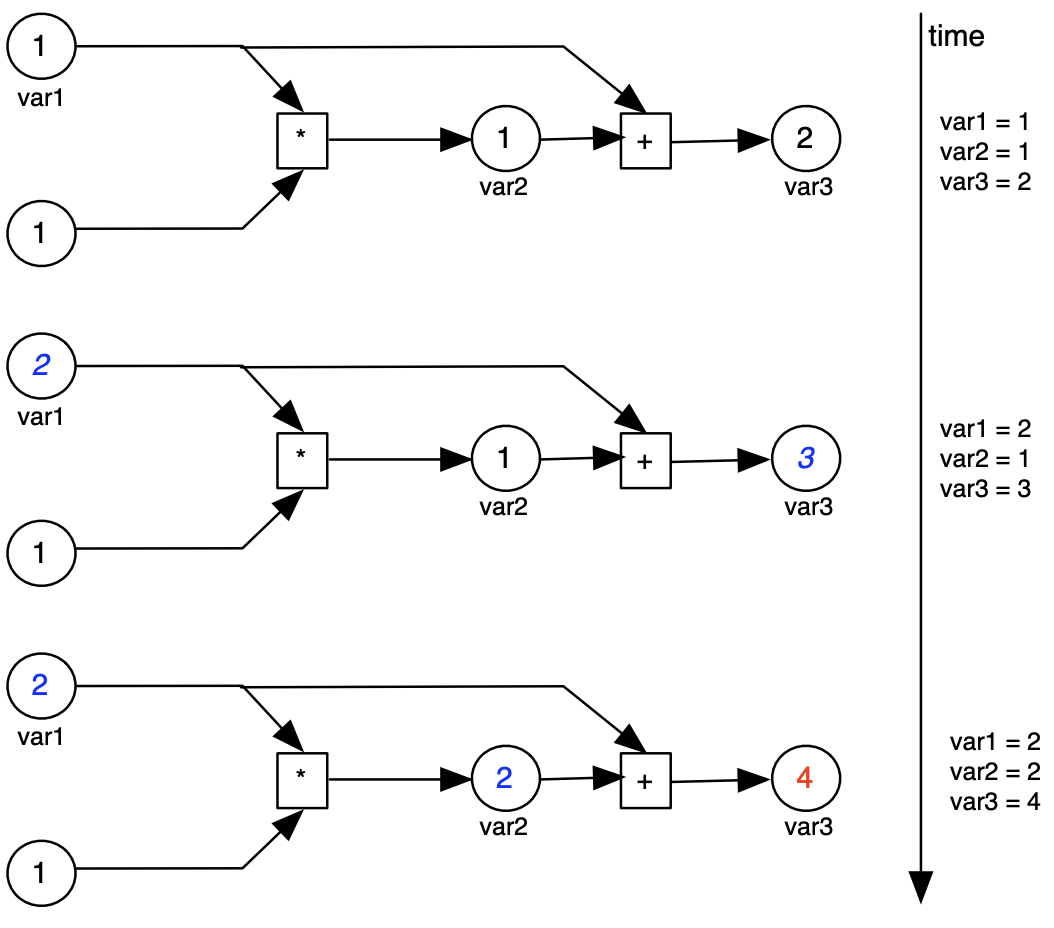
\includegraphics[width=.65\linewidth]{figures/reactive-programming/RP-glitch.png}
    \caption{Rappresentazione di un possibile glitch nella programmazione reattiva \cite{DBLP:journals/csur/BainomugishaCCMM13}.}
    \label{fig:rp-glitch}
\end{figure}

La maggior parte dei linguaggi di programmazione reattiva elimina i glitch organizzando le espressioni in un grafo ordinato topologicamente, garantendo così che un'espressione venga sempre valutata dopo che tutte le dipendenze sono state valutate. 
Nella teoria dei grafi l'ordinamento topologico di un grafo consiste nell'ordinare linearmente i suoi nodi in modo che preso un qualunque arco $xy$ dal nodo $x$ al nodo $y$, $x$ venga prima di $y$ nell'ordinamento. In altre parole, i nodi sono disposti in modo tale che ognuno di essi preceda tutti i nodi collegati ai suoi archi uscenti seguendo l'ordinamento scelto.
Le implementazioni reattive più recenti riescono ad evitare i glitch nei programmi reattivi eseguiti su un singolo computer, ma non nei programmi reattivi distribuiti. Evitare problemi in un ambiente distribuito non è un'attività banale a causa dei guasti di rete, ritardi e mancanza di un orologio globale.

\section{Lifting}
Quando la programmazione reattiva è incorporata nei linguaggi host (come libreria o come estensione), gli operatori esistenti (ad esempio + o *) e le funzioni o i metodi definiti dall'utente devono essere convertiti per operare con le astrazioni di base di essa. 
La conversione di un operatore ordinario in una variante in grado di operare con valori che possono variare nel tempo è nota come \textit{lifting}. 
Esistono diverse strategie per effettuare il lifting: 
\begin{itemize}
    \item \textbf{lifting implicito}: viene effettuata una trasformazioebe automatica di operazioni su singoli valori in operazioni su flussi di valori senza la necessità di scrivere codice per gestire questa trasformazione. Il lifting implicito rende la programmazione reattiva trasparente agli utilizzatori. 
    \item \textbf{lifting esplicito}: in questo caso il linguaggio fornisce una serie di primitive che possono essere utilizzate per effettuare il lifting.
    \item \textbf{lifting manuale}: il linguaggio non fornisce operatori per effettuare il lifting. Il programmatore deve ottenere manualmente il valore corrente di un valore variabile nel tempo, che poi può essere utilizzato con gli operatori del linguaggio. 
\end{itemize}

\section{Entità osservabili e osservatrici}
Nel contesto della programmazione reattiva, le fonti di dati o eventi che emettono informazioni vengono chiamate \textbf{entità osservabili}, mentre le \textbf{entità osservatrici} sono quelle che si collegano a queste fonti per monitorare e reagire ai dati o agli eventi emessi. In questa sezione vengono descritte le due entità, evidenziando le loro caratteristiche. 
\subsection{Entità osservabile}
Un'entità osservabile rappresenta un flusso continuo di dati o eventi che può essere emesso in modo regolare o completamente asincrono. Questo flusso può essere caratterizzato da una quantità variabile di elementi, incluso zero, uno o un numero infinito di essi. Questo concetto è fondamentale per gestire dati in tempo reale le interazioni utente in applicazioni moderne, consentendo una gestione dinamica dei flussi di informazioni.

Tuttavia, l'entità osservabile va oltre la semplice emissione di dati o eventi. Essa può concludersi in due modi principali: notificando un completamento avvenuto o segnalando un errore anomalo durante la sua esecuzione. Il completamento avvenuto è tipicamente utilizzato quando il flusso di dati ha termini definiti e finiti, ad esempio dopo il completamento di una sequenza di operazioni. D'altra parte, l'errore può essere segnalato in caso di malfunzionamenti imprevisti, come errori di connessione di rete o eccezioni di programmazione.

Se consideriamo un'entità osservabile con un flusso infinito di elementi, come ad esempio gli eventi di click dell'utente in un'applicazione Android, è importante notare che non sarà mai in grado di emettere un messaggio di completamento, questo perché il completamento è riservato solo al termine naturale del flusso di eventi disponibili, il quale, se infinito, non si verifica mai. Tuttavia, è possibile che l'entità osservabile termini in modo anomalo, segnalando un errore, nel caso si verifichino anomalie durante la sua esecuzione. In tal caso, l'entità osservabile con un flusso infinito terminerà anticipatamente e non emetterà ulteriori elementi.

\subsection{Entità Osservatrice}
Un'entità osservatrice può instaurare una connessione (sottoscrizione) con un'entità osservabile al fine di monitorare e gestire i dati o gli eventi trasmessi da quest'ultima secondo specifiche politiche reattive. 
Gli elementi all'interno di un flusso sono emessi in modo sequenziale, uno dopo l'altro, e vengono elaborati dall'entità osservatrice in modo consecutivo. Questa caratteristica impedisce la comparsa di corse critiche, mantenendo l'ordine delle operazioni e garantendo una gestione reattiva dei dati.
Nel caso in cui un grande numero di dati o eventi venga emesso rapidamente dall'entità osservabile e l'entità osservatrice non sia in grado di elaborarli con la stessa velocità, è possibile adottare strategie come l'utilizzo di una \textit{coda degli eventi} o il meccanismo di \textit{buffering} per gestire in modo efficiente il flusso di dati e prevenire perdite o sovraccarichi.
Un'entità osservabile può essere sottoscritta da zero, una o più entità osservatrici contemporaneamente, permettendo una gestione flessibile e dinamica del flusso di dati o eventi all'interno di un'applicazione reattiva. 

\section{Programmazione reattiva distribuita}
Un linguaggio per la programmazione reattiva distribuita permette la ripartizione dei dati e del grafo delle dipendenze computazionali fra più nodi di una rete in un ambiente distribuito. 
Prendendo come esempio l'espressione \texttt{var3 = var1 + var2}, le tre variabili e il relativo grafo delle dipendenze potrebbero trovarsi su nodi diversi della rete. 

La progettazione di un linguaggio reattivo distribuito è di gran lunga più complessa rispetto ad un linguaggio reattivo tradizionale. La principale difficoltà risiede nel fatto che in questi contesti occorre considerare fattori come latenza, congestione della rete, guasti di essa e la mancanza di un orologio globale. Un linguaggio reattivo distribuito, come già anticipato in~\Cref{sec:glitch}, non riesce a garantire la completa rimozione delle inconsistenze dei dati nel grafo delle dipendenze, portando quindi a glitch. La presenza di un grafo delle dipendenze in un programma reattivo distribuito, oltre a portare alla presenza di glitch, tende ad accoppiare strettamente i componenti dell'applicazione, rendendoli quindi meno resistenti ad errori e riducendone la scalabilità complessiva~\cite{DBLP:journals/programming/MyterSM19}. 
Una soluzione che potrebbe essere adottata è utilizzare un approccio centralizzato, nel quale un'entità avente un orologio centrale è responsabile dell'ordinamento degli aggiornamenti nel grafo delle dipendenze. Questo approccio introduce un \textit{singolo punto di rottura} e un eccessivo numero di comunicazioni dovute al fatto che tutte le parti coinvolte devono comunicare con una singola entità ogni qualvolta ricevono e propagano dati, limitando in questo modo la scalabilità dell'architettura. 

\section{Il Manifesto Reattivo}
Il 16 settembre 2014 è stata rilasciata la seconda versione del \textit{Manifesto Reattivo}~\footnote{https://www.reactivemanifesto.org/}, un documento redatto da esperti del settore tra cui Jonas Bonér, Dave Farley, Roland Kuhn e Martin Thompson. Questo manifesto, piuttosto che essere un trattato sulla programmazione reattiva, si presenta come una guida pratica per la progettazione di sistemi reattivi, delineando le caratteristiche chiave che tali sistemi dovrebbero possedere.
È importante comprendere che il manifesto non promuove un'unica metodologia o paradigma di programmazione reattiva, ma piuttosto si concentra su principi generali che possono essere applicati a una vasta gamma di architetture e tecnologie. L'obiettivo è garantire che i sistemi reattivi siano capaci di affrontare sfide come la scalabilità, la resilienza e la responsività, comuni nell'ambito delle applicazioni moderne.
La necessità di redigere il manifesto è stata spinta dai rapidi cambiamenti nel panorama tecnologico. Mentre in passato le applicazioni erano caratterizzate da un'architettura monolitica, tempi di risposta relativamente lunghi e gestione di volumi limitati di dati, oggi vi è una realtà in cui le applicazioni devono essere distribuite su una vasta gamma di dispositivi, supportare grandi volumi di dati e fornire risposte quasi istantanee agli utenti.
Gli autori del manifesto descrivono un sistema reattivo come \textbf{flessibile}, a \textbf{basso accoppiamento} e \textbf{scalabile}: questo lo rende più semplice da sviluppare e più malleabile nel tempo. Tali sistemi sono più \textbf{tolleranti ai guasti} e reagiscono ad essi in modo elegante e non brusco. Sono altamente \textbf{responsivi}, offrendo agli utenti un feedback concreto.
Il manifesto delinea quattro principali caratteristiche, rappresentate in~\Cref{fig:rp-reactive-manifesto}, che un sistema deve assolutamente possedere per essere considerato reattivo: 
\begin{itemize}
    \item \textbf{responsività}: il sistema, se è in generale possible dare una risposta ai client, la dà in maniera tempestiva. La responsività è la pietra miliare dell'usabilità e dell'utilità del sistema; essa presuppone che i problemi vengano identificati velocemente e gestiti in modo efficace. I sistemi responsivi sono focalizzati a minimizzare il tempo di risposta, individuando per esso un limite massimo prestabilito di modo da garantire una qualità del servizio consistente nel tempo. Il comportamento risultante è quindi predicibile, il che semplifica la gestione delle situazioni di errore, genera fiducia negli utenti finali e predispone ad ulteriori interazioni con il sistema;
    \item \textbf{relisienza}: il sistema resta responsivo anche in caso di guasti. Ciò riguarda non solo i sistemi ad alta disponibilità o mission-critical, infatti, accade che ogni sistema che non è resiliente si dimostrerà anche non responsivo in seguito ad un guasto. La resilienza si acquisisce tramite replica, contenimento, isolamento e delega. I guasti sono relegati all'interno di ogni componente, isolando così ogni componente dagli altri e quindi garantendo che il guasto delle singole porzioni del sistema non comprometta il sistema intero. Il recupero di ogni componente viene delegato ad un altro componente (esterno) e l'alta disponibilità viene assicurata tramite replica laddove necessario. I client di un componente vengono dunque alleviati dal compito di gestirne i guasti;
    \item \textbf{elasticità}: il sistema rimane responsivo sotto carichi di lavoro variabili nel tempo. I sistemi reattivi possono adattarsi alle variazioni nella frequenza temporale degli input incrementando o decrementando le risorse allocate al processamento degli stessi. Questo porta ad architetture che non hanno né sezioni contese né colli di bottiglia, favorendo così la distribuibilità o la replica dei componenti e la ripartizione degli input su di essi. I sistemi reattivi permettono l'implementazione predittiva, oltre che reattiva, di algoritmi scalabili perché fondati sulla misurazione real-time della performance. Tali sistemi, raggiungono l'elasticità in maniera cost-effective su commodity hardware e piattaforme software a basso costo;
    \item \textbf{orientato ai messaggi}: i sistemi reattivi si basano sullo scambio di messaggi asincrono per delineare per ogni componente il giusto confine che possa garantirne il basso accoppiamento con gli altri, l'isolamento e la trasparenza sul dislocamento e permetta di esprimere i guasti del componente sotto forma di messaggi al fine di delegarne la gestione. L'utilizzo di uno scambio esplicito di messaggi permette migliore gestibilità del carico di lavoro, elasticità e controllo dei flussi di messaggi mediante setup e monitoraggio di code di messaggi all'interno del sistema. Uno scambio di messaggi trasparente rispetto al dislocamento rende possibile, ai fini della gestione dei guasti, l'utilizzo degli stessi costrutti e semantiche sia su cluster che su singoli host. Uno stile di comunicazione non bloccante fa sì che l'entità ricevente possa solo consumare le risorse, il che porta ad un minor sovraccarico sul sistema.
\end{itemize}

\begin{figure}
    \centering
    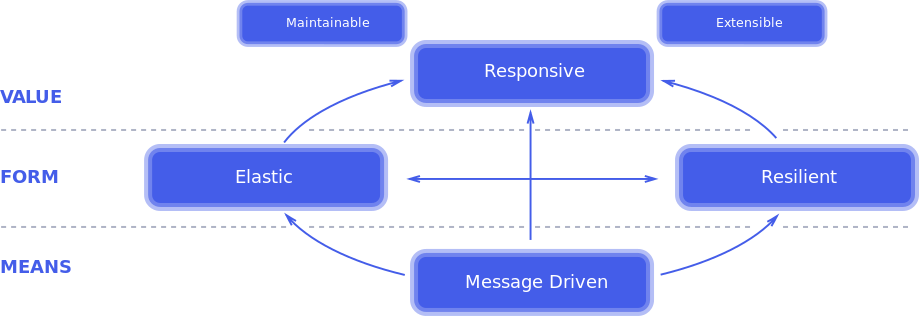
\includegraphics[width=.80\linewidth]{figures/reactive-programming/reactive-manifesto.png}
    \caption{Caratteristiche fondamentali di un sistema reattivo.}
    \label{fig:rp-reactive-manifesto}
\end{figure}


%----------------------------------------------------------------------------------------
% Programmazione reattiva in kotlin
%----------------------------------------------------------------------------------------
\chapter{Programmazione reattiva in Kotlin}
\section{Kotlin}
\textbf{Kotlin}~\footnote{https://kotlinlang.org/} è un linguaggio di programmazione, sviluppato dall'azienda JetBrains~\footnote{https://www.jetbrains.com/} nel 2011, il quale si pone come alternativa a linguaggi come Java e Scala, che girano su \textit{Java Virtual Machine} (JVM). La crescita di Kotlin è stata piuttosto rapida, affermandosi come linguaggio di programmazione di riferimento per applicazioni Android. 
È possibile configurare Kotlin per essere eseguito su JVM, ma può essere compilato anche in codice Javascript o direttamente in nativo tramite la struttura di compilazione LLVM~\cite{DBLP:conf/lcpc/LattnerA04} per essere eseguito su dispositivi Android. 
Kotlin è un linguaggio a tipizzazione statica che unisce i costrutti tipici della programmazione ad oggetti con alcuni di quelli della programmazione funzionale. 
Una delle caratteristiche principali di Kotlin è la sua \textbf{concisione} ed \textbf{espressività}: in media è necessario scrivere il 40\% di codice in meno rispetto alla controparte Java per raggiungere le stesse funzionalità. Questo è possibile poiché i pattern più comuni sono supportati di default a livello di linguaggio. 
Un'altra caratteristica fondamentale è la \textbf{null-safety}. In Kotlin i tipi definiscono se un oggetto può essere nullo o meno. Inoltre Kotlin è tipizzato staticamente, ciò significa che tutti i tipi sono conoscibili a tempo di compilazione, siano essi dichiarati esplicitamente o inferiti dal compilatore stesso. Gli eventuali errori vengono quindi intercettati prima dell'esecuzione del codice. 
Il codice scritto in Kotlin è interoperabile con il codice scritto in linguaggio Java. È possibile quindi richiamare codice Kotlin da codice Java e viceversa.

\section{Coroutines}
Sebbene siano utilizzate da oltre 50 anni, non esiste una definizione universale su cosa sia una \textit{coroutine}. 
Kotlin definisce una coroutine come un'istanza di una \textit{suspending function}, ovvero una funzione che può sospendere temporaneamente la propria esecuzione, concettualmente simile ad un \textit{thread}, per il fatto che entrambi prendono un blocco di codice da eseguire e hanno un ciclo di vita simile. Le coroutines tuttavia, non sono limitate ad un singolo thread. La loro esecuzione può essere sospesa in un thread e può essere ripristinata in un altro. 

\subsection{Classificazione}
Ana Lucia De Moura e Roberto Ierusalimschy~\cite{DBLP:journals/toplas/MouraI09} classificano le coroutines secondo la loro implementazione: 
\begin{itemize}
    \item \textbf{trasferimento del controllo simmetrico/asimmetrico}: riguarda il modo in cui le coroutines gestiscono il flusso di esecuzione e la comunicazione con altre coroutines o con il thread principale.
    Nel trasferimento del controllo \textit{simmetrico}, le coroutine cooperano tra loro per controllare l'esecuzione. Le coroutines con trasferimento del controllo simmetrico sono generalmente implementate utilizzando un meccanismo cooperativo, dove una coroutine può essere sospesa e ripresa solo quando decide di farlo.
    D'altra parte, nel trasferimento del controllo \textit{asimmetrico}, una delle coroutines coinvolte detiene il controllo sull'esecuzione e può assegnarlo ad altre coroutines in modo asincrono. In questo modello, una coroutine può essere sospesa o ripresa anche senza il suo consenso diretto, poiché il controllo è gestito in modo asincrono dal sistema o da un'entità esterna;
    \item \textbf{implementazione stackful/stackless}: influenza il modo in cui vengono gestite le coroutines e la profondità dello stack delle chiamate.
    In un'implementazione \textit{stackful}, ogni coroutine ha il proprio stack separato, simile a quello di un \textit{thread}. Ciò consente a ciascuna di esse di eseguire chiamate ricorsive senza causare un \textit{overflow} dello stack, poiché ogni coroutine ha il proprio stack dedicato. Tuttavia, questo approccio richiede una gestione importante delle risorse, poiché ogni coroutine richiede un'allocazione di memoria separata per lo stack.
    In un'implementazione \textit{stackless}, le coroutines condividono lo stesso stack o utilizzano un modello di gestione dello stack non ricorsivo, come i \textit{coroutine frames}. Questo modello rende la gestione delle coroutine più efficiente in termini di utilizzo delle risorse, ma può limitare la profondità delle chiamate ricorsive e potenzialmente causare un overflow dello stack se la profondità delle chiamate è troppo grande; 
    \item \textbf{supporto di prima classe/limitato}: influisce sul grado di flessibilità e controllo che gli sviluppatori hanno quando utilizzano le coroutines.
    Con il \textit{supporto di prima classe}, le coroutines sono trattate come qualsiasi altro tipo di dato nel linguaggio di programmazione. Ciò significa che possono essere passate come argomenti a funzioni, restituite come valori di ritorno da funzioni e assegnate a variabili.
    Il \textit{supporto limitato} per le coroutine porta a restrizioni sulle operazioni che è possibile eseguire con le coroutines.
\end{itemize}


\subsection{Limitazioni della programmazione asincrona}
\label{sec:async-limitation}
La programmazione asincrona è soggetta agli stessi problemi della programmazione in generale; allo stesso tempo, presenta una serie di problemi unici, non rilevanti per il codice sincrono~\cite{DBLP:conf/oopsla/ElizarovBAU21}. In questa sezione verranno discussi brevemente due dei problemi che influenzano maggiormente lo spazio di progettazione per un linguaggio di programmazione con supporto alla programmazione asincrona: ``\textbf{colorazione delle funzioni}'' e \textbf{gestione degli errori}.

\subsubsection{Colorazione delle funzioni}
Una differenza importante tra diverse implementazioni di computazione asincrona riguarda la gestione della divisione tra codice asincrono e sincrono. Ci si riferisce a questo problema come ``\textit{colorazione delle funzioni}''.
Questo è un concetto comune che assume diverse forme e formalizzazioni, ma in sostanza si riduce a un numero di regole semplici: 
\begin{itemize}
    \item ogni programma o funzione è assegnata ad un particolare colore, ad esempio rosso o blu; 
    \item il codice blu rappresenta la computazione sincrona e può essere acceduto da entrambi i colori; 
    \item il codice rosso rappresenta invece la computazione asincrona, e può essere acceduto solo dal codice di colore rosso;  
    \item esistono costrutti speciali che consentono di chiamare il codice rosso da quello blu, in alternativa, il codice delle \textit{entry function} è rosso. 
\end{itemize}
Per risolvere questo problema si potrebbe pensare ad un linguaggio in cui tutto il codice è rosso, e tutte le computazioni sono quindi asincrone. Nella realtà, però, introdurre computazione asincrona in tutte le funzioni porta a diversi problemi: 
\begin{itemize}
    \item la computazione asincrona introduce complessità rispetto alla chiamata di normali funzioni;
    \item molti linguaggi di programmazione sono sincroni per natura e introducono costrutti asincroni solo per determinati scopi. La mancanza di una chiara distinzione tra funzioni sincrone e asincrone porta a problemi di comprensione del programma;
    \item La gestione degli errori e la loro propagazione in codice rosso è un task particolarmente complesso. Se tutto il codice fosse rosso, sarebbe richiesto una gestione avanzata degli errori in tutto il codice.  
\end{itemize}


\subsubsection{Gestione degli errori}
Un altro problema cruciale nella programmazione asincrona riguarda la gestione degli errori. Quando si hanno più esecuzioni asincrone in corso contemporaneamente e una di esse fallisce, il modo per recuperare e proseguire l'esecuzione non è così lineare come nel codice sincrono. Nel codice standard, esiste una chiara relazione tra chiamante e chiamato: gli errori nel chiamato si propagano verso l'alto al chiamante e vengono gestiti lì o continuano a propagarsi. Tuttavia, nel codice asincrono, questa relazione non è più presente e senza di essa non c'è un punto di responsabilità definito su chi debba gestire quali errori. È anche possibile che sia necessario propagare la gestione degli errori verso il basso, ad esempio per annullare calcoli non necessari.
Per affrontare questo problema, si possono utilizzare le funzionalità offerte dal linguaggio di programmazione per creare un meccanismo di gestione degli errori sostitutivo, tuttavia, tutte queste soluzioni non sono ottimali per la gestione degli errori verso il basso.
Un approccio più strutturato alla gestione degli errori asincroni incorporerebbe sia la gestione verso l'alto che quella verso il basso. 

Esistono due approcci principali utilizzati nella programmazione asincrona attuale. Il primo si basa sugli \textbf{alberi di supervisione}. Questo metodo prevede l'organizzazione esplicita delle attività asincrone in alberi padre-figlio, che corrispondono alla struttura desiderata di propagazione degli errori verso l'alto e verso il basso. In caso di errore, è possibile scegliere se isolare, propagare o riavviare il sotto-albero di attività interessato. Il secondo approccio è chiamato \textbf{concorrenza strutturata}, propone di applicare i principi della programmazione strutturata alla programmazione asincrona. In questo caso, se un'attività A avvia un'attività B, la durata di B non può superare quella di A. Questo schema stabilisce una relazione di ``\textit{launcher-launchee}'' invece di quella \textit{chiamante-chiamato} e descrive come propagare gli errori e le cancellazioni verso il basso.
Rispetto agli alberi di supervisione, la concorrenza strutturata è meno flessibile, poiché la strategia di gestione degli errori è predefinita. Tuttavia, è anche meno verbosa e corrisponde meglio al modo in cui solitamente viene scritto il codice asincrono.

\subsection{Goals}
Kotlin è stato concepito come un linguaggio di programmazione pragmatico, pensato per essere utilizzato quotidianamente e per agevolare gli sviluppatori nel completare i loro compiti attraverso le sue funzionalità e strumenti. Questo stesso approccio viene applicato al suo supporto per la programmazione asincrona, con obiettivi principali ben definiti.

Prima di tutto, Kotlin mira a garantire \textbf{l'indipendenza dalle specifiche implementazioni di basso livello} delle piattaforme. Poiché è progettato per essere un linguaggio multipiattaforma, costruire un supporto asincrono basato su altre implementazioni (come ad esempio i futures su JVM) potrebbe generare diversi problemi, soprattutto in termini di interoperabilità tra le diverse piattaforme.

Inoltre, Kotlin si impegna a essere altamente \textbf{adattabile alle implementazioni esistenti}. Essendo relativamente nuovo, il linguaggio presta particolare attenzione all'interoperabilità con il codice già esistente, con un'enfasi speciale sul lavoro con il codice Java sulla piattaforma JVM in modo trasparente. Considerando che esistono già approcci consolidati per la gestione del codice asincrono su piattaforme specifiche (come ad esempio le promise in JavaScript o le operazioni di input/output non bloccanti su JVM), Kotlin mira a integrare senza soluzione di continuità tali API nel suo ecosistema.

Infine, Kotlin punta a fornire un \textbf{supporto per la programmazione asincrona pragmatica}. L'avvento e la diffusione dell'approccio async/await, rispetto ad altri stili di programmazione asincrona, hanno evidenziato l'importanza della leggibilità del codice. Anche se l'approccio async/await potrebbe essere meno espressivo rispetto a quello basato sulle coroutine, copre la maggior parte dei casi d'uso pratici e offre anche prestazioni migliori.

\subsection{Coroutine builder}
I \textbf{coroutine builder} sono funzioni che consentono di creare e avviare coroutine in Kotlin. In Kotlin sono disponibili diversi coroutine builder, i più utilizzati sono:
\begin{itemize}
    \item \textbf{launch}: è utilizzato per avviare una nuova coroutine in modo asincrono. Quando si utilizza \textit{launch}, la coroutine viene avviata e viene eseguito il codice all'interno della coroutine in modo indipendente dal flusso principale del programma. Questo significa che la coroutine può essere eseguita in background senza bloccare il thread principale.
    \textit{Launch} non restituisce alcun valore, quindi è utilizzato principalmente per operazioni di tipo \textit{fire-and-forget}; 
    l'esecuzione ritorna un oggetto \texttt{job}, sul quale si può eseguire il metodo \texttt{join()}, che blocca il thread chiamante fino a quando la coroutine non è terminata. 
    Le eccezioni che accadono in una coroutine eseguita con \textit{launch} sono propagate alla coroutine padre, ma non alle coroutines sorelle. Se viene lanciata una eccezione e non viene gestita, questa verrà ignorata silenziosamente. 
    \item \textbf{async}: è utilizzato per avviare una coroutine che restituisce un valore, cioè un'operazione che produce un risultato. A differenza di \textit{launch}, \textit{async} restituisce un oggetto \texttt{Deferred}, che rappresenta il risultato futuro dell'operazione asincrona. Il valore può essere ottenuto utilizzando la funzione \texttt{await()} su un oggetto \texttt{Deferred}. Anche in questo caso il thread chiamante è bloccato finché non è stato prodotto il risultato. 
    Questo è utile quando si desidera eseguire un'operazione asincrona e recuperare il risultato prodotto da essa.
    Le eccezioni in questo caso sono immagazzinate all'interno dell'oggetto \texttt{Deferred}. Se eseguiamo il metodo \texttt{await()}, l'eccezione viene rilanciata e può essere gestita con un normale blocco \texttt{try-cath} o altri meccanismi di gestione delle eccezioni. 
    \item \textbf{runBlocking}: è un coroutine builder che fa da ponte fra il codice al suo interno e il mondo esterno alle coroutine. Il thread che esegue questo builder viene bloccato per tutta la durata della chiamata, finché tutte le coroutine al suo interno non hanno completato la loro esecuzione. 
\end{itemize}

\subsection{Coroutine scope e concorrenza strutturata}
Un \textbf{coroutine scope} fornisce un modo per gestire il ciclo di vita delle coroutines, consentendo di avviare, gestire o cancellare gruppi di coroutines in modo coerente e sicuro. Ciascuna di esse deve essere gestita all'interno di uno scope e quando questo viene cancellato tutte le coroutines al suo interno vengono cancellate. I coroutine scope possono essere nidificati, in questo caso quando uno scope di livello superiore viene cancellato, vengono cancellate tutte le coroutines al suo interno e tutti gli scope interni vengono cancellati ricorsivamente. La radice di questo albero di dipendenze è chiamata \texttt{GlobalScope}. Anche se è possibile eseguire le coroutines all'interno dello scope globale, è consigliato creare nuovi scope secondo la necessità e renderli figli e genitori l'uno dell'altro in modo logico, sicuro e efficiente. 
In sintesi, il coroutine scope permette di gestire le coroutines in modo strutturato, definendo il ciclo di vita delle stesse. Questo garantisce che le risorse vengano gestite in modo corretto e che le attività vengano terminate in modo ordinato, migliorando l'affidabilità e la manutenibilità del software e risolvendo i problemi della gestione degli errori nella programmazione asincrona descritti nella~\Cref{sec:async-limitation}

\subsection{Coroutine context}
Il \textbf{coroutine context} è un insieme persistente di oggetti definiti dall'utente che possono essere associati alla coroutine stessa. Questo insieme può includere oggetti responsabili delle politiche di threading della coroutine, del logging, degli aspetti di sicurezza e di transazione dell'esecuzione della coroutine, nonché dell'identità e del nome della stessa.
Se pensiamo alle coroutines come thread leggeri, il contesto di una coroutine può essere paragonato a una raccolta di variabili locali del thread. Tuttavia, a differenza delle variabili locali del thread, il contesto di una coroutine è immutabile, ma è possibile aggiungerne elementi usando l'operatore \texttt{plus}. Questo non rappresenta una grave limitazione, poiché le coroutines sono così leggere che è facile lanciarne una nuova quando c'è la necessità di modificare qualcosa nel contesto.
La libreria standard non include implementazioni concrete, ma fornisce un'interfaccia, consultabile al Listato~\ref{lst:coroutine-contex-interface}, in modo che tutti questi aspetti possano essere definiti in modo componibile. 
Concettualmente, il coroutine context può essere considerato una sorta di ibrido tra un insieme e una mappa: gli elementi hanno chiavi come in una mappa, ma le chiavi sono direttamente associate agli elementi, similmente ad un insieme.
Ogni elemento di un coroutine context è esso stesso un contesto. Questo consente la creazione di contesti composti.
In~\Cref{fig:rp-coroutine-context} è possibile notare come lo scope di una coroutine figlio venga definito partire dal contesto dello scope padre e aggiungendo la propria istanza di \texttt{job}. 

\begin{figure}
    \centering
    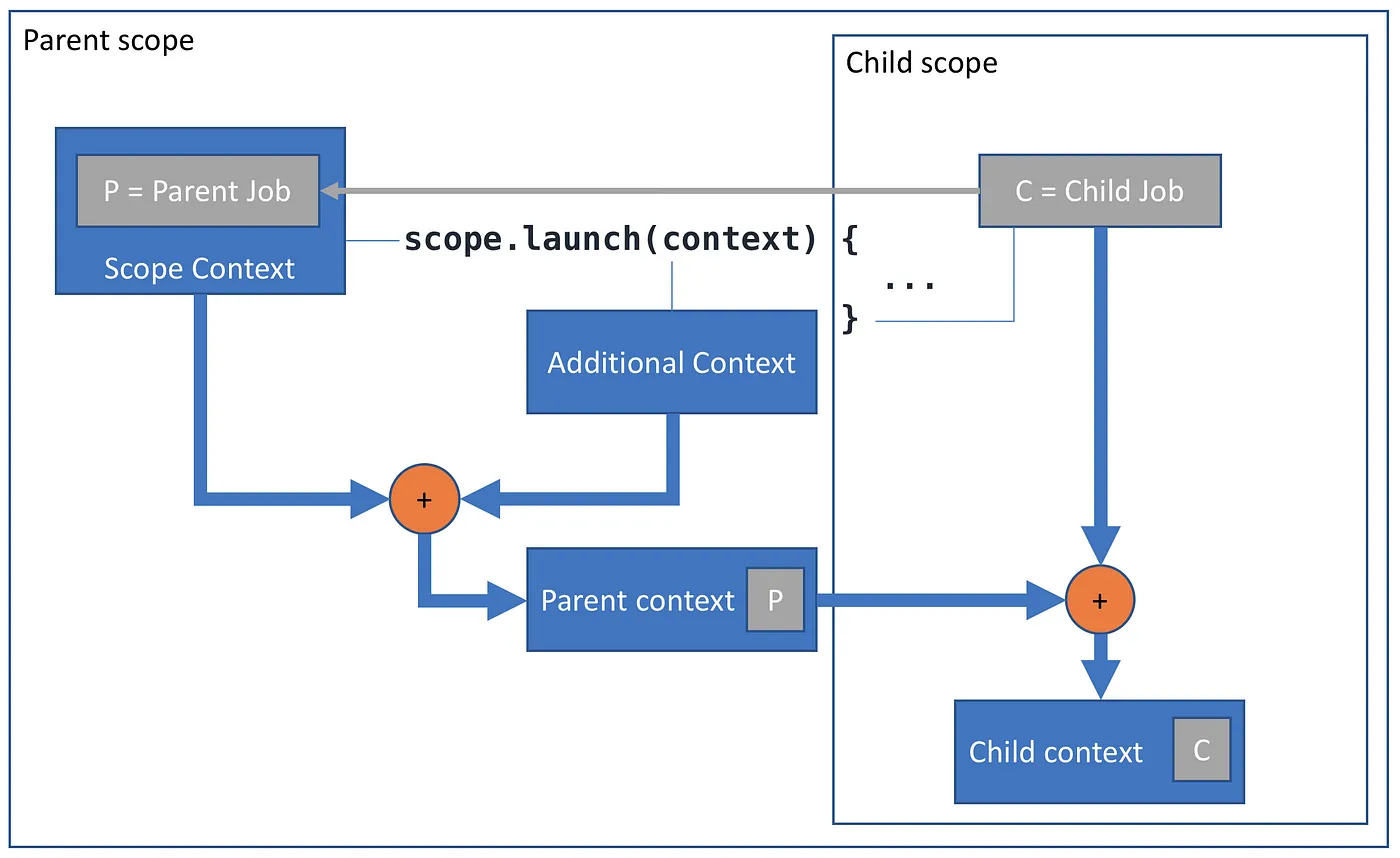
\includegraphics[width=.80\linewidth]{figures/reactive-programming/coroutine-context.png}
    \caption{La nuova coroutine crea la propria istanza di \texttt{job} e definisce il proprio contesto a partire dal contesto padre più il job creato.}
    \label{fig:rp-coroutine-context}
\end{figure}

\lstinputlisting[float,language=Kotlin,caption = {Interfaccia definita per il coroutine context, presente nel package \texttt{kotlin.coroutines}.}, label={lst:coroutine-contex-interface}]{listings/coroutines/coroutine-context.kt}

\subsubsection{Coroutine Dispatcher}
Un coroutine context include un \textbf{coroutine dispatcher}, il quale determina quale o quali thread saranno utilizzati per l'esecuzione delle coroutine. È responsabile dell'allocazione delle risorse di sistema necessarie per l'esecuzione delle coroutines e della coordinazione del loro funzionamento su thread o altri thread pool disponibili nel sistema.
I dispatchers più comuni disponibili in Kotlin sono: 
\begin{itemize}
    \item \textbf{Dispatchers.Default}: viene utilizzato per eseguire le coroutine su un pool di thread con un numero di thread pari al numero di processori disponibili nel sistema o un multiplo di esso. È adatto per operazioni di CPU-bound, come elaborazioni intensive o calcoli.
    \item \textbf{Dispatchers.IO}:  viene utilizzato per eseguire le coroutines su un pool di thread dedicato alle operazioni I/O-bound, come operazioni di lettura/scrittura su file, operazioni di rete, o chiamate API. Questo dispatcher ha un pool di thread più grande rispetto a Dispatchers.Default per consentire un numero maggiore di operazioni di I/O contemporaneamente.
    \item \textbf{Dispatchers.Main}: è specifico per le applicazioni Android e viene utilizzato per eseguire le coroutine sul thread principale della User Interface (UI). È importante utilizzare questo dispatcher quando si effettuano operazioni che coinvolgono l'interfaccia utente per evitare blocchi o rallentamenti dell'UI.
    \item \textbf{Dispatchers.Unconfined}: Questo dispatcher esegue le coroutine in modo sequenziale sul thread chiamante, senza alcun thread pool dedicato. È utile in situazioni in cui si desidera eseguire il codice sul  thread chiamante fino a quando non è necessario passare ad un altro thread.
\end{itemize}
Tutti i coroutine builder, come \texttt{launch} e \texttt{async}, accettano opzionalmente un coroutine context come parametro che può essere usato per specificare esplicitamente il dispatcher e altri elementi per la nuova coroutine. 
Quando un coroutine builder è utilizzato senza parametri, eredita il contesto (e quindi il dispatcher) dal coroutine scope dal quale è stato eseguito. 

\section{Kotlin Flow}
Kotlin flow è una libreria che offre un'API reattiva per gestire i flussi di dati asincroni in applicazioni Kotlin. Basato sul modello della programmazione reattiva, Kotlin Flow permette agli sviluppatori di creare, trasformare e combinare flussi di eventi in modo dichiarativo e componibile.
Android descrive un flow come un tipo in grado di emettere valori in sequenza, a differenza delle suspending function, le quale restituiscono un solo valore. È possibile per esempio utilizzare un flow per ricevere aggiornamenti in tempo reale da un database. Concettualmente un flow è un flusso di dati che può essere consumato in modo asincrono. 
Un flow è molto simile ad un iteratore che produce una sequenza di valori, ma utilizza suspending function per produrre e consumare valori in modo asincrono. 
Le entità coinvolte nei flow sono tre: 
\begin{itemize}
    \item \textbf{produttore}: produce i dati che sono aggiunti al flusso; 
    \item \textbf{intermediario} (opzionale): può modificare ogni valore emesso nel flusso o il flusso stesso senza consumare i valori; 
    \item \textbf{consumatore}: consuma i valori dal flusso. 
\end{itemize}

\subsection{Tipi di flow}
Nel contesto dei Kotlin Flow, possiamo dividere i flussi in due categorie: \textbf{cold flow} e \textbf{hot flow}. 
I cold flow emettono valori sono quando avviene una sottoscrizione. Ogni qualvolta un osservatore si sottoscrive ad un cold flow viene avviata la produzione dei valori dall'inizio del flusso di dati. Ogni sottoscrizione a questo tipo di flow ha quindi il proprio flusso di dati privato, il quale è indipendente dagli altri. 
Un hot flow, al contrario, emette valori continuamente, indipendentemente dalla presenza o meno di sottoscrizioni attive. Quando un osservatore si sottoscrive a un hot flow, inizia a ricevere i valori emessi da quel momento in avanti, senza influenzare la produzione dei valori stessi. Non esistono flussi privati per ciascuna sottoscrizione, quindi tutti gli osservatori ricevono gli stessi valori emessi. 

\subsubsection{Cold Flow}
\label{sec:cold-flow}
Come è possibile notare in~\Cref{fig:rp-flow-class-diagram}, tutti i tipi di flow estendono dall'interfaccia \textit{Flow}, il cui codice è consultabile al Listato~\ref{fig:rp-flow-interface}.
L'interfaccia \texttt{Flow} ha un solo metodo \texttt{collect(collector: FlowCollector<T>)}. 
Quando utilizziamo i flow builder, i quali saranno introdotti successivamente, come \texttt{asFlow()} o \texttt{flowOf()}, in realtà stiamo chiamando una funzione chiamata \texttt{flow()}, la quale accetta una lambda come parametro. Questa lambda ha come ricevitore implicito un \texttt{FlowCollector}, che è un'interfaccia contenente il solo metodo \texttt{emit}.
Quindi possiamo chiamare direttamente il metodo \texttt{emit} su questa lambda per emettere valori nel flusso. Ad esempio, quando utilizziamo \texttt{Iterable.asFlow()}, per ogni elemento dell'iterabile, internamente viene chiamato il metodo \texttt{emit} per emettere il valore all'interno del flusso.
Kotlin permette questa sintassi grazie alla \textit{Single Abstract Method conversion} (SAM conversion), che consente di passare una lambda direttamente dove è richiesto un oggetto di un'interfaccia funzionale.
Quindi, quando collezioniamo i valori di un flusso utilizzando il metodo \texttt{collect}, in realtà stiamo invocando la lambda che abbiamo definito precedentemente all'interno di flow, e ogni volta che questa lambda viene eseguita, i valori vengono riemessi sul flusso utilizzando il metodo \texttt{emit}.

\lstinputlisting[float,language=Kotlin,caption = {Codice dell'interfaccia Flow}, label = {fig:rp-flow-interface}]{listings/flow/flow.kt}

\begin{figure}
    \centering
    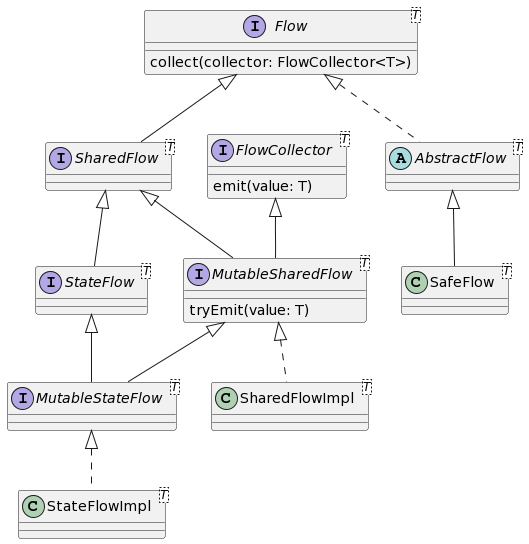
\includegraphics[width=.80\linewidth]{figures/reactive-programming/flow-class-diagram.png}
    \caption{Diagramma delle classi dei Kotlin Flow.}
    \label{fig:rp-flow-class-diagram}
\end{figure}

\subsubsection{Hot Flow}
\label{sec:hot-flow}
Come anticipato, a differenza dei cold flow, i quali riemettono tutti i valori ad ogni nuova sottoscrizione, gli hot flow emettono elementi in continuazione. 
Esistono due tipi di hot flow: \textbf{sharedFlow} e \textbf{stateFlow}. 
In questo caso a livello implementativo sia l'emissione che la collezione degli elementi funziona in maniera leggermente differente rispetto ai cold flow. 

\paragraph{SharedFlow}
Uno SharedFlow rappresenta un flusso di dati condiviso che può essere letto da più collector contemporaneamente. È prevalentemente utilizzato quando si desidera condividere flussi di dati tra più parti dell'applicazione. 
Internamente, SharedFlow ha un \textit{buffer} in grado di mantenere valori che saranno poi collezionati dagli osservatori. 
Quando uno sharedFlow viene dichiarato, è possibile settare il parametro \texttt{replay}, il quale definisce il numeri di valori precedenti che vengono emessi ai nuovi collector all'atto della sottoscrizione. Ad esempio, se \texttt{replay} è settato a 2, il flusso emetterà gli ultimi due valori ai nuovi collector. 
Un altro parametro che è possibile settare è \texttt{extraBufferCapacity}, il quale è utile per permettere agli osservatori più lenti di ricevere i valori senza sospendere gli emettitori. 
L'ultimo parametro è \texttt{onBufferOverflow}, utile per scegliere la strategia con la quale gestire l'emissione di nuovi elementi in caso di \textit{buffer overflow}. 
Quando un produttore invoca il metodo \texttt{emit}, il valore viene aggiunto al buffer. 
Il metodo \texttt{collect}, come è possibile notare nel Listato~\ref{fig:rp-sharedflow-collect}, esegue un \texttt{ciclo while} che non termina mai, il che significa che il metodo \texttt{collect} è bloccante e perciò necessita di essere eseguito in una coroutine dedicata. 
Ad ogni iterazione, viene controllato se esiste un nuovo valore da collezionare. Se questo esiste viene richiamato il metodo \texttt{emit} proprio come nel caso dei cold flow, descritti nella~\Cref{sec:cold-flow}. 

\lstinputlisting[float,language=Kotlin,caption = {Codice delL'implementazione del metodo collect negli sharedFlow.}, label = {fig:rp-sharedflow-collect}]{listings/flow/shared-flow-collect.kt}

\paragraph{StateFlow}
Uno StateFlow rappresenta uno stato in sola lettura con un singolo valore aggiornabile che emette aggiornamenti ai suoi collector. È particolarmente utile quando è necessario rappresentare qualsiasi tipo di stato. 
A differenza dello SharedFlow, non ha un buffer interno. Lo stato viene gestito tramite un campo \texttt{value}, il quale viene sovrascritto ad ogni cambiamento di stato. 
Questa caratteristica impedisce ai consumatori troppo lenti di leggere tutti gli elementi emessi sul flusso. Infatti, nel caso di due emissioni consecutive sul flow, un osservatore troppo lento potrebbe accorgersi solo dell'ultimo stato. 
Per dichiarare uno StateFlow è necessario settare uno stato iniziale. 
Quando viene invocato il metodo \texttt{emit} da un produttore, in realtà quello che accade è l'aggiornamento del campo \texttt{value}. 
Per quando riguarda la raccolta degli elementi, possiamo notare nel Listato~\ref{fig:rp-stateflow-collect}, che il metodo \texttt{collect} è anche in questo caso un metodo bloccante, e che per controllare la disponibilità di nuovi valori, effettua un confronto fra il vecchio stato e quello attualmente presente nel campo \texttt{value}. 

\lstinputlisting[float,language=Kotlin,caption = {odice delL'implementazione del metodo collect negli stateFlow.}, label = {fig:rp-stateflow-collect}]{listings/flow/state-flow-collect.kt}

\subsection{Creazione di un flusso}
Esistono diversi modi per inizializzare un flow, alcune dei metodi principali: 

    \begin{itemize}
        \item \textbf{cold flow}: 
        \begin{itemize}
            \item \texttt{flowOf()}: è possibile creare un flow fornendo una serie di valori come argomenti. 
            \item \texttt{asFlow()}: serve per convertire una collezione, come ad esempio una lista, in un flow. 
            \item \texttt{flow\string{\string}}: è possibile creare un flow emettendo direttamente i valori all'interno della lambda. 
        \end{itemize}
        \item \textbf{hot flow}: 
        \begin{itemize}
            \item \texttt{mutableSharedFlow<T>()}: per dichiarare uno SharedFlow occorre specificare il tipo di dato del flusso. 
            \item \texttt{mutableStateFlow(value)}: per inizializzare uno StateFlow è necessario fornire un valore iniziale. 
        \end{itemize}
    \end{itemize}
   

Esempi di codice per inizializzare un flow sono disponibili al Listato~\ref{lst:flow-builder}.

\lstinputlisting[float,language=Kotlin,caption = {Esempi di come i flow builder possono essere utilizzati per inizializzare nuovi flow.}, label={lst:flow-builder}]{listings/flow/flow-builder.kt}

\subsection{Operatori}
Gli operatori sono funzioni specializzate progettate per manipolare, trasformare e controllare i flussi. Gli operatori possono essere divisi in due categorie principali: 
\begin{itemize}
    \item \textbf{operatori intermediari}: permettono di manipolare il flusso, consentendo di creare pipeline di operazioni che verranno eseguite solo quando si attiva un operatore di terminazione. Gli operatori intermedi includono: 
    \begin{itemize}
        \item operatori di trasformazione come \textbf{map}, \textbf{flatmap} e \textbf{transform}; 
        \item operatori di filtraggio come \textbf{filter}, \textbf{distinct} e \textbf{take}; 
        \item operatori di combinazione come \textbf{zip} e \textbf{combine};
        \item operatori di gestione degli errori come \textbf{catch} e \textbf{retry};
        \item operatori di gestione del tempo come \textbf{debounce};
    
    \end{itemize}
    \item \textbf{operatori di terminazione}: il comportamento di un operatore di terminazione è differente per quanto riguarda hot flows e cold flows. In un cold flow ogni sottoscrizione riavvia l'emissione dei dati dall'inizio della sorgente dati. Un operatore di terminazione quindi avvia l'esecuzione del flusso. In un hot flow, i dati sono già in corso di generazione, indipendentemente dalla presenza di sottoscrizioni. In questo caso un operatore di terminazione consente di iniziare a consumare i dati da qualsiasi punto essi si trovino, senza riavviare l'emissione dall'inizio. 
    Gli operatori di terminazione includono: 
    \begin{itemize}
        \item \textbf{collect}: consuma i valori emessi dal flusso e li elabora. 
        \item \textbf{toList, toSet, toMap}: raccolgono i valori emessi dal flusso e li convertono nella collezione desiderata. 
        \item \textbf{reduce, fold}: riducono e aggregano rispettivamente i valori emessi dal flusso in un singolo valore. 
    \end{itemize}
\end{itemize}

%----------------------------------------------------------------------------------------
% Progettazione e implementazione del prototipo
%----------------------------------------------------------------------------------------
\chapter{Progettazione e implementazione del prototipo}
\section{Scelta delle tecnologie}
Come linguaggio di programmazione per lo sviluppo del prototipo è stato scelto \textbf{Kotlin}. Le ragioni principali di questa decisione sono: 
\begin{itemize}
    \item \textbf{continuità con il codice preesistente}: il simulatore Alchemist, nel quale si intende integrare la soluzione, è stato inizialmente sviluppato utilizzando il linguaggio Java. Tuttavia, nel corso del tempo, lo sviluppo è stato portato avanti utilizzando Kotlin.  Questa transizione può essere stata motivata da diverse ragioni, tra cui la maggior espressività e la maggiore sicurezza del codice offerte da Kotlin rispetto a Java. Perciò, per mantenere la coerenza e la continuità con il codice già esistente, è logico che il prototipo venga sviluppato utilizzando Kotlin;
    \item \textbf{vantaggi di Kotlin}: Kotlin è un linguaggio di programmazione moderno che offre numerosi vantaggi rispetto a Java. Tra questi vantaggi vi sono la concisione della sintassi, la null safety integrata, la gestione migliorata delle eccezioni e molte altre caratteristiche che consentono di scrivere codice più pulito, sicuro ed efficiente. Utilizzare Kotlin per lo sviluppo del prototipo permetterà quindi di beneficiare di queste caratteristiche, migliorando la produttività e la qualità del codice;
    \item \textbf{interoperabilità con Java}: un altro punto importante da considerare è l'interoperabilità di Kotlin con Java. Essendo entrambi i linguaggi compatibili con la JVM, è possibile utilizzare liberamente librerie Java esistenti all'interno del codice Kotlin e viceversa. Questo significa che il prototipo sviluppato in Kotlin potrà facilmente integrarsi con il codice Java esistente nel simulatore Alchemist, sfruttando le funzionalità e le risorse già disponibili senza doverle riscrivere o adattare.
\end{itemize}

Per quando riguarda la libreria reattiva, è stata scelta \textbf{Kotlin Flow} rispetto all'alternativa \textbf{RxKotlin}. Questa decisione è stata presa considerando diversi fattori e vantaggi: 
\begin{itemize}
    \item \textbf{integrazione nativa con Kotlin}: Kotlin Flow è parte integrante della libreria standard di Kotlin, mentre RxKotlin è una libreria esterna. Kotlin Flow si integra quindi più naturalmente con il codice Kotlin e sfrutta le caratteristiche specifiche del linguaggio in modo più efficace;
    \item \textbf{supporto per la programmazione asincrona strutturata}: Kotlin Flow è progettato per supportare la programmazione asincrona strutturata, facilitando la gestione di flussi di dati reattivi in modo più chiaro e intuitivo;
    \item \textbf{gestione delle risorse}: Kotlin Flow offre un meccanismo integrato per la gestione delle risorse, consentendo di gestire automaticamente la chiusura delle risorse quando non sono più necessarie;
    \item \textbf{compatibilità con coroutine}: Kotlin Flow è completamente compatibile con le coroutines di Kotlin, consentendo di combinare facilmente flussi reattivi con il modello asincrono basato su coroutine. 
\end{itemize}

\section{Progettazione}
\label{sec:progettazione}
Trattandosi dello sviluppo di un prototipo, avente come fine ultimo quello dell'integrazione nel simulatore Alchemist, è stato scelto di mantenere lo stesso modello del dominio, astraendo però dalla metafora chimica presente in Alchemist, descritta in~\Cref{sec:alchemist}. 
A seguito di questa scelta, nel modello del dominio del prototipo non esiste il concetto di \textbf{reazione}, il quale viene sostituito con il concetto di \textbf{evento}. Non esiste nemmeno il concetto di \textbf{molecola}, il quale è sostituito da un generico \textbf{content}. Restano invariati invece gli altri concetti. 
Come si può notare in figura, l'\textbf{environment} contiene al suo interno un insieme di \textbf{nodi} e tutti i \textbf{vicinati}, i quali vengono creati grazie ad una regola di collegamento (\textbf{linking rule}). L'environment è anche responsabile di mantenere la \textbf{posizione} di ciascun nodo, consentirne l'aggiunta, la rimozione e lo spostamento. 
Ogni nodo ha al suo interno \textbf{eventi}, i quali possono verificarsi ad un determinato istante, e \textbf{content}, ovvero contenitori di valori. 
Ogni evento a sua volta contiene \textbf{condizioni}, le quali devono essere soddisfatte per garantire l'esecuzione dell'evento stesso, e le \textbf{azioni} che verranno eseguite a seguito della sua esecuzione.
Ogni evento ha anche un \textbf{tempo putativo}, ovvero il tempo al quale è schedulata la sua prossima occorrenza.
È possibile osservare il modello appena descritto in~\Cref{fig:design-class-diagram}.

\begin{figure}
    \centering
    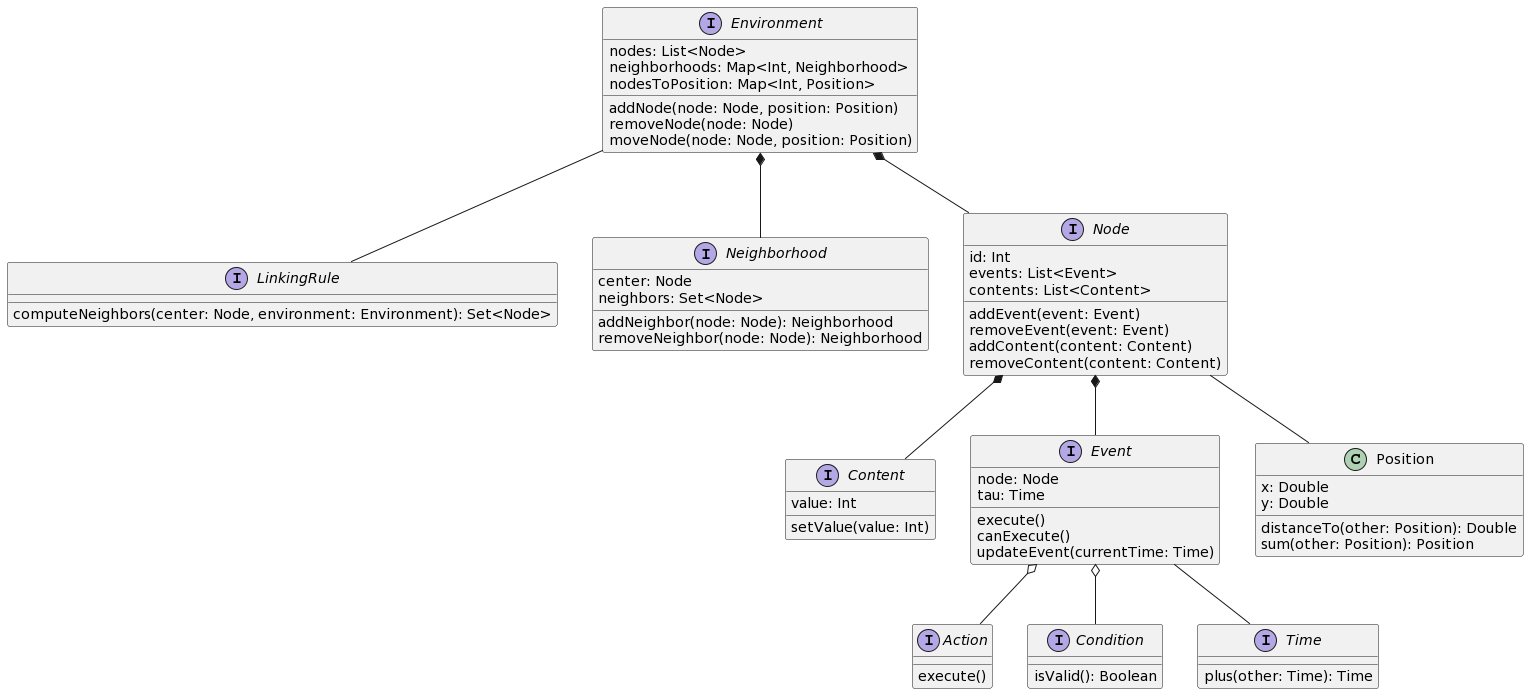
\includegraphics[width=\linewidth]{figures/design/class-diagram.png}
    \caption{Design del modello del dominio.}
    \label{fig:design-class-diagram}
\end{figure}

È stata prevista anche la presenza di un \textbf{engine}, ovvero il motore della simulazione, responsabile di far partire la simulazione e farla avanzare, e di uno \textbf{scheduler}, responsabile di mantenere una lista degli eventi futuri, ordinati per tempo di accadimento. 

\subsection{Eliminazione grafo delle dipendenze}
Come anticipato in sezione~\Cref{sec:alchemist}, Alchemist gestisce le dipendenze fra gli eventi utilizzando un grafo delle dipendenze, nel quale i nodi sono le reazioni (eventi) e gli archi connettono una reazione $r$ a tutti i nodi che dipendono da essa, ovvero quelli il cui tempo di attivazione deve essere aggiornato a seguito dell'esecuzione di $r$. 
L'utilizzo di un grafo delle dipendenze in un simulatore ad eventi discreti per l'aggiornamento degli eventi dipendenti richiede elevata capacità di calcolo, specialmente quando il sistema presenta una complessità elevata o un grande numero di eventi da gestire.
Per affrontare la complessità computazionale derivante dalla gestione di un grafo delle dipendenze è stato scelto di eliminare tale grafo, optando invece per un approccio basato sulla programmazione reattiva. In questo contesto, ogni evento osserva gli eventi da cui dipende e reagisce di conseguenza aggiornando il proprio tempo di occorrenza, riducendo così la necessità di una gestione esplicita delle dipendenze tramite grafo. Un evento può osservare gli altri eventi presenti all'interno dello stesso nodo e gli eventi presenti nei nodi del vicinato. 
Utilizzando la programmazione reattiva, gli eventi possono essere modellati come flussi di dati che si propagano attraverso il sistema. Ogni evento può essere definito come un'unità indipendente che reagisce ai cambiamenti negli eventi osservati, senza la necessità di mantenere un grafo delle dipendenze centralizzato. 
Poiché eventi e nodi possono essere rimossi dall'environment e i vicini possono cambiare in base alla regola di collegamento scelta, è fondamentale riconoscere che l'insieme di eventi osservati da un singolo evento può variare durante l'esecuzione della simulazione. Pertanto, oltre agli eventi da cui dipende direttamente, un evento deve essere in grado di reagire ai cambiamenti nell'insieme degli eventi presenti nel suo nodo, nonché ai cambiamenti nei nodi del suo vicinato.  

\subsection{Gestione dei cambiamenti nell'ambiente}
\label{sec:linking-rule}
Come anticipato in precedenza, la creazione dei vicinati è affidata alla \textit{linking rule}, la quale ne definisce le regole per la creazione. La creazione dei vicinati può essere eseguita osservando la posizione dei nodi nell'\textit{environment}, i valori dei content all'interno dei nodi stessi, o altre parti arbitrarie dell'environment. 
Per far fronte alla complessità della creazione e dell'aggiornamento dei vicinati, è stato scelto di adottare un approccio basato sulla programmazione reattiva. Ciò significa che la linking rule è implementata in modo da osservare reattivamente l'ambiente circostante e reagire di conseguenza agli eventi che coinvolgono i nodi.
In pratica, la linking rule monitora ciò di cui ha bisogno per la creazione dei vicinati e osserva l'insieme dei nodi presenti nell'environment in modo da rilevarne eventuali modifiche come l'aggiunta o la rimozione e aggiornare di conseguenza i vicinati dei nodi interessati. Potrebbe essere necessario osservare altri attributi dei nodi, come i valori contenuti al loro interno, per definire in modo più preciso i vicinati.
Per esempio, se i vicinati vengono definiti in base alla loro posizione, occorre osservarne anche il cambiamento di posizione durante la simulazione.

\section{Implementazione}
Nel contesto di una simulazione è importante che gli osservatori ricevano tutti lo stesso stato al fine di garantire la coerenza dei risultati. Si è deciso quindi di utilizzare flow di tipo hot, descritti in~\Cref{sec:hot-flow}. 
Come descritto precedentemente, i possibili hot flow utilizzabili nella libreria Kotlin Flow sono \textbf{MutableSharedFlow} e \textbf{MutableStateFlow}. Si è scelto di utilizzare i primi nel caso in cui il flusso dovesse rappresentare lo stato attuale di una determinata risorsa, mentre i secondi sono stati utilizzati nel caso in cui si volesse comunicare un determinato evento che è accaduto all'interno della simulazione. Le scelte in dettaglio verranno analizzate successivamente nel capitolo. 

\subsection{Criticità nell'uso degli Hot Flow in simulazioni a step}
In una simulazione a step è essenziale garantire uno stato consistente prima di procedere allo step successivo al fine di garantire risultati accurati ed affidabili. 
L'utilizzo degli hot flow, con la loro natura asincrona e non deterministica, rende difficile garantire questa consistenza dello stato, poiché non esiste un momento definito in cui tutti gli osservatori hanno elaborato i dati e lo stato è completamente aggiornato. 
Come anticipato in~\Cref{sec:hot-flow}, la chiamata alla funzione \texttt{collect}, la quale controlla costantemente la presenza di nuovi elementi da consumare, non termina mai ed è quindi necessario eseguire ciascuna di esse in una coroutine dedicata. Questa coroutine, rimarrà attiva fino al termine della simulazione, o fino a quando l'osservatore necessiterà dei dati emessi su tale flusso. 
Quando un nuovo elemento viene emesso su un flusso hot, non è possibile controllare con precisione quando tutti gli osservatori hanno finito di elaborare il nuovo elemento; il controllo ritorna al punto di emissione del flusso non appena tutti gli osservatori lo hanno ricevuto. Ci si potrebbe quindi trovare nella situazione in cui inizia un nuovo step senza che gli aggiornamenti degli eventi dipendenti o la creazione dei nuovi vicinati sia stata effettivamente terminata. 
Ogni osservatore, oltretutto, può a sua volta reagire alla presenza di un elemento su un flusso, emettendo a sua volta elementi su un altro flusso, creando così un albero di chiamate asincrone che può diventare complesso da gestire e sincronizzare. 

Nel contesto di questo prototipo, il termine dello step non è il solo punto in cui è necessaria consistenza nello stato del sistema. Come è stato descritto in~\Cref{sec:progettazione}, l'occorrenza di un evento scatena l'esecuzione di una o più azioni, le quali potrebbero necessitare dello stato attuale dell'ambiente per prendere decisioni su come modificarlo. 
Un altro punto nel quale è necessaria consistenza è quando un evento intende notificare gli eventi da esso dipendenti della sua effettiva esecuzione. Qui la consistenza è necessaria poiché le azioni eseguite potrebbero aver modificato la topologia dei vicinati, portando quindi ad una variazione nella lista degli eventi dal quale ogni singolo evento dipende. 
La garanzia che tutti gli eventi dipendenti abbiano aggiornato il proprio tempo putativo prima di proseguire con lo step successivo è fondamentale per garantire che la lista di eventi futuri sia ordinata nel modo corretto. Quando si gestisce una simulazione a step, è essenziale mantenere un controllo accurato del tempo e degli eventi che devono accadere in specifici momenti temporali. Se un evento dovesse aggiornare il suo tempo dopo la fine dello step in cui dovrebbe effettivamente farlo, potrebbe causare un problema di inconsistenza temporale nell'ambiente di simulazione.
Si immagini di avere un evento programmato per accadere in un certo momento temporale all'interno di uno step. Dopo la fine di questo step, l'evento potrebbe aggiornare il suo tempo per essere pianificato per il prossimo step. Tuttavia, se questo aggiornamento non avviene correttamente, potrebbe verificarsi una situazione in cui, al successivo step, l'evento si ritrovi nella lista degli eventi futuri con un tempo minore rispetto al tempo corrente.

\subsection{Soluzione al problema}
Come spiegato precedentemente il problema principale risiede nel fatto che la libreria Kotlin Flow non mette a disposizione meccanismi per controllare l'avvenuto consumo di un elemento pubblicato sul flusso. Si è deciso quindi di implementare un meccanismo per risolvere questa necessità. 
L'idea di base è fare in modo che a seguito di ogni emissione sul flusso, si attenda una notifica da parte degli osservatori dell'avvenuta consumazione dell'elemento. Così facendo, il controllo torna all'entità che ha emesso sul flusso solo quando tutti gli osservatori hanno effettivamente consumato l'elemento. Utilizzando questo approccio non occorre preoccuparsi di possibili alberi di chiamate asincrone, poiché, nel caso in cui un osservatore emettesse elementi a sua volta su un ulteriore flusso, anch'esso aspetterebbe le notifiche dai consumatori di tale flusso, e il controllo tornerebbe all'emettitore alla radice solo quando tutto l'albero è stato risolto con successo.
Per fare ciò, si sono utilizzate due classi ad-hoc: \textit{AwaitableMutableStateFlow} e \textit{AwaitableMutableSharedFlow}, il cui codice è disponibile al Listato~\ref{lst:awaitable-mutable-flow}. Le suddette classi implementano rispettivamente le interfacce \textit{MutableStateFlow} e \textit{MutableSharedFlow}, delegando però l'effettiva implementazione a \textit{StateFlowImpl} e \textit{SharedFlowImpl}. Entrambe le classi implementate eseguono l'\textit{override} del metodo \texttt{emit}, aggiungendo la logica per attendere le notifica descritta sopra, e definiscono il metodo \texttt{notifyConsumed}, utilizzato dall'osservatore per comunicare l'effettivo consumo dell'elemento. La logica per attendere il consumo degli elementi emessi è incapsulata all'interno del flow stesso, l'attesa è perciò trasparente lato emettitore. È stata creata anche una classe astratta \textit{AbstractAwaitableMutableFlow}, la quale è estesa da entrambe le classi implementate, per evitare ripetizione di codice. 
In~\Cref{fig:extended-flow} è possibile notare come le classi implementate appena descritte si interfacciano con le classi definite nella libreria Kotlin Flow. 


\begin{figure}
    \centering
    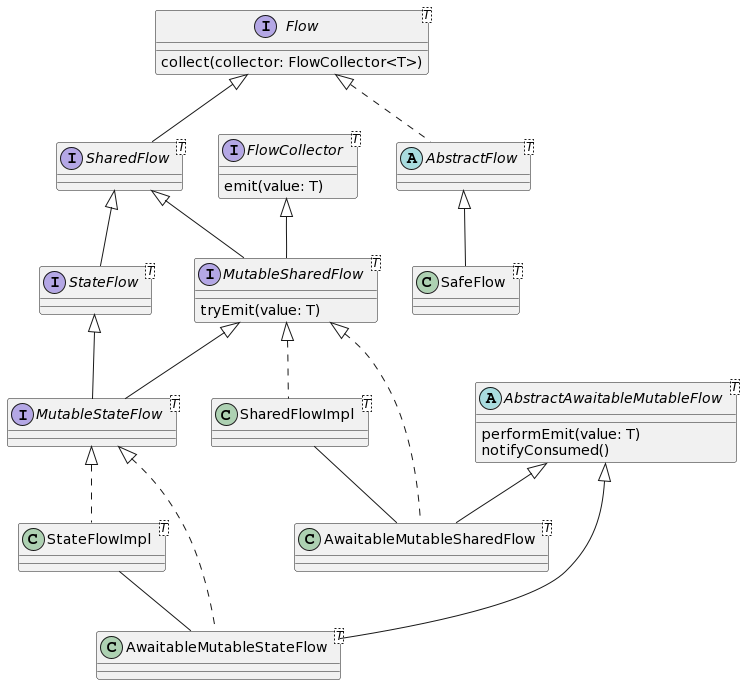
\includegraphics[width=\linewidth]{figures/implementation/extended-flow.png}
    \caption{Diagramma delle classi dei Kotlin Flow estesa con le classi implementate ad-hoc.}
    \label{fig:extended-flow}
\end{figure}

\lstinputlisting[float,language=Kotlin,caption = {Implementazione delle classi \textit{AwaitableMutableFlow}.}, label={lst:awaitable-mutable-flow}]{listings/implementation/awaitableMutableFlow.kt}

\subsection{Gestione reattiva dipendenze fra eventi}
In seguito si intende descrivere come tramite la programmazione reattiva si è implementata la gestione delle dipendenze fra eventi. 
Come anticipato, ogni evento è dipendente dagli eventi che accadono all'interno dello stesso nodo e dagli eventi che accadono nei nodi del vicinato. La natura di questo insieme di eventi è dinamica, poiché durante la simulazione nodi ed eventi possono essere rimossi e la topologia del vicinato può cambiare. 
Ciascun evento, tiene traccia degli eventi da cui dipende tramite l'utilizzo di due mappe, entrambe aventi come chiave l'evento osservato e come valore il \texttt{job} associato alla coroutine nella quale è stata avviata l'osservazione. La prima mappa, \textit{observedLocalEvents}, tiene traccia degli eventi locali al nodo, mentre la seconda tiene traccia degli eventi appartenenti ai nodi del vicinato. 
Come si può notare nel Listato~\ref{lst:observe-local-events}, ciascun evento si mette in ascolto in attesa di cambiamenti nella lista degli eventi presenti nel nodo in cui risiede. Ad ogni cambiamento, inizia ad osservare nuovi eventi aggiunti e smette di osservare gli eventi che sono stati rimossi. 
Nel Listato~\ref{lst:observe-neighbor-events}, invece, è consultabile il codice riferito all'osservazione degli eventi presenti nei nodi facenti parte il vicinato.

\lstinputlisting[float,language=Kotlin,caption = {Codice utilizzato per l'osservazione degli eventi locali al nodo.}, label={lst:observe-local-events}]{listings/implementation/observeLocalEvents.kt}

\lstinputlisting[float,language=Kotlin,caption = {Codice utilizzato per l'osservazione degli eventi presenti nei nodi del vicinato}, label={lst:observe-neighbor-events}]{listings/implementation/observeNeighborEvents.kt}

\subsection{Gestione reattiva aggiornamento dell'environment}
Come specificato in~\Cref{sec:linking-rule}, per aggiornare i vicinati, la \textit{linking rule} deve osservare i cambiamenti nella lista dei nodi presenti all'interno dell'environment e, a seconda della strategia di creazione dei vicinati scelta, altre parti arbitrarie dell'environment. 
All'interno del prototipo è possibile trovare l'implementazione di una linking rule che crea i vicinati in base alla posizione dei nodi nell'environment. Ciò non toglie la possibilità di aggiungere altre strategie al simulatore e scegliere ad ogni simulazione la strategia desiderata. 
Nel Listato~\ref{lst:observe-environment} è presente il codice con il quale la classe \textit{Position Linking Rule} osserva la lista di nodi presenti nell'environment e la loro posizione all'interno di esso, ricreando ogni volta i vicinati corretti. 

\lstinputlisting[float,language=Kotlin,caption = {Codice utilizzato per l'osservazione dei nodi presenti all'interno dell'environment e della loro posizione.}, label={lst:observe-environment}]{listings/implementation/observeEnvironment.kt}

\subsection{Fase di inizializzazione degli osservatori}
Utilizzando flussi hot, occorre una fase di sincronizzazione iniziale nella la quale vi sia la certezza che al termine della creazione dell'istanza di un osservatore, qualunque esso sia, esso sia pronto immediatamente a collezionare gli elementi.
Questa necessità è data dal fatto che, come descritto in precedenza, ogni osservazione viene eseguita all'interno di una coroutine separata, e pertanto il controllo del flusso torna immediatamente al chiamante, il quale potrebbe emettere elementi prima che l'osservatore sia effettivamente pronto per collezionarli. 
Per ovviare a tale problema si è fatto uso del metodo \texttt{onSubscription}, fornito da \textit{SharedFlow} e \textit{StateFlow}. Il metodo in questione viene invocato quando la connessione al flow da parte dell'osservatore è stata effettivamente stabilita e consente di definire azioni da eseguire in quel determinato momento.
In fase di inizializzazione dell'osservatore viene inizializzato un \textit{CountDownLatch}, il cui valore è pari al numero di flow su cui l'osservatore dovrà mettersi in ascolto. 
Al momento di ogni effettiva sottoscrizione viene decrementato il latch. 
Così facendo si ha la certezza che una volta terminata l'inizializzazione di un osservatore, questo sia effettivamente pronto per consumare gli elementi emessi sul flow. 

\subsection{Engine e scheduler}
L'\textit{engine}, come spiegato in~\Cref{sec:progettazione}, è responsabile di far partire la simulazione e del suo avanzamento. In fase di inizializzazione aggiorna il tempo putativo degli eventi presenti nell'environment, dopodiché li aggiunge allo scheduler. 
Una volta terminata la fase di inizializzazione fa partire l'effettiva simulazione, la quale termina nel caso in cui sia stato raggiunto il limite massimo di step eseguibili o non ci sia più nessun evento programmato per essere eseguito. 
Ad ogni step della simulazione, l'\textit{engine}:
\begin{enumerate}
    \item preleva, se presente, il prossimo evento da eseguire dallo scheduler;
    \item aggiorna il tempo della simulazione con il tempo dell'evento da eseguire;
    \item controlla che le condizioni dell'evento da eseguire siano soddisfatte;
    \item esegue effettivamente l'evento;
    \item aggiorna il tempo putativo dell'evento appena eseguito;
    \item comunica allo scheduler di ordinare la lista di eventi futuri, poiché i tempi putativi di alcuni eventi potrebbero essere cambiati. 
\end{enumerate}
Si noti che, a seguito della chiamata per eseguire l'evento, il controllo ritorna all'engine solo nel momento in cui tutte le azioni dell'evento sono state effettivamente eseguite, tutte le dipendenze fra eventi sono state aggiornate e gli eventi dipendenti da quello eseguito hanno aggiornato il proprio tempo putativo. 
Il codice utilizzato per al gestione del singolo step appena descritto è consultabile al Listato~\ref{lst:engine-step}. 
In questa fase prototipale è stato scelto di implementare lo \textit{scheduler} di eventi attraverso una semplice lista. Se il prototipo dovesse poi essere integrato nel simulatore Alchemist, questa soluzione sarebbe limitante dal punto di vista delle performance, poiché ad ogni step, viene effettuato un ordinamento completo della lista di eventi, in tal caso si renderebbe necessario l'utilizzo di meccanismi più efficienti, come quello già presente in Alchemist, descritto in~\Cref{sec:next-reaction-method}.

\lstinputlisting[float,language=Kotlin,caption = {Codice per l'esecuzione di un singolo step all'interno della simulazione.}, label={lst:engine-step}]{listings/implementation/engineStep.kt}


\section{Considerazioni sui risultati raggiunti}
Il prototipo sviluppato è stato concepito con l'intento di essere poi integrato all'interno del simulatore Alchemist. Prima di immergersi nella fase di sviluppo del codice per Alchemist, è stato ritenuto fondamentale dedicare del tempo alla valutazione preliminare della fattibilità di tale progetto. Questo approccio ha permesso di acquisire una comprensione approfondita dei requisiti tecnici, delle possibili criticità e delle opportunita associate all'integrazione. 
Tuttavia, dato che si tratta di un prototipo, è importante sottolineare che esso astrae la complessità presente in Alchemist. Questo significa che al momento risultata difficile effettuare un confronto diretto fra la soluzione presentata e il simulatore. Eventuali valutazioni delle performance dovranno essere effettuate una volta completata l'integrazione. 
L'implementazione della programmazione reattiva, caratterizzata da un flusso di lavoro asincrono, ha portato alla luce alcune criticità quando è stata combinata con la simulazione a step. In una simulazione a step, è fondamentale mantenere la consistenza dell'ambiente, specialmente prima di procedere allo step successivo. La natura asincrona della programmazione reattiva può causare situazioni in cui gli eventi vengono elaborati in tempi variabili, rendendo difficile garantire che lo stato dell'ambiente sia coerente e stabile. Si potrebbe definire l'approccio adottato per risolvere tale problema come un ``work around''. Questo perché la programmazione reattiva mira a gestire gli eventi in modo asincrono, senza dover attendere il completamento di un'operazione prima di procedere con altre attività. Aspettare che tutti gli osservatori consumino un elemento introduce una dipendenza sincrona che può rallentare l'esecuzione complessiva del programma.

\subsection{Possibili miglioramenti}
Trattandosi di un prototipo, avente come obiettivo l'analisi della fattibilità della creazione di un simulatore ad eventi discreti le cui dipendenze e aggiornamento dell'environment avvenissero in maniera reattiva, alcuni aspetti legati soprattutto alle performance sono stati trascurati. Questi aspetti, in sede di integrazione con il simulatore Alchemist dovranno sicuramente essere presi in considerazione per la riuscita del progetto. 
Uno dei punti che si è scelto di trascurare è la creazione dei vicinati da parte della \textit{linking rule}. Attualmente essa, ad ogni cambiamento al quale è interessata, ricrea tutti i vicinati a partire dalle informazioni dei nodi dell'environment. Ovviamente questa scelta non è ottimale dal punto di vista delle performance. Per migliorare ciò si potrebbe prendere in considerazione l'aggiornamento dei vicinati solo dei nodi interessati. Questo miglioramento richiede che la linking rule mantenga internamente uno stato corrente di ciò a cui è interessata, e una volta ricevuto l'aggiornamento, capisca autonomamente quali sono stati i cambiamenti. 
Un'altra implementazione piuttosto ``naive'' è quella dello scheduler, responsabile di mantenere una lista ordinata dei prossimi eventi da eseguire. 
Utilizzare una semplice lista, che verrà riordinata ad ogni step, porta a problemi di performance, soprattutto in casi in cui il numero di eventi futuri è piuttosto elevato. 
Implementazioni come quella attualmente presente nel simulatore Alchemist sono sicuramente più efficienti. 


%----------------------------------------------------------------------------------------
% Conclusioni
%----------------------------------------------------------------------------------------
\chapter{Conclusioni}
In questa tesi è stata eseguita una panoramica sulle simulazioni ad eventi discreti e sulla programmazione reattiva, in generale e applicata al linguaggio Kotlin. 
Il prodotto della tesi condotta è la prototipazione di un simulatore ad eventi discreti reattivo. Il prototipo segue la modellazione del dominio presente in Alchemist, nel quale dovranno poi essere integrate le funzionalità sviluppate, eliminando la necessità del grafo delle dipendenze fra eventi, utilizzando tecniche di programmazione reattiva al fine di rendere implicite queste dipendenze. La programmazione reattiva è stata utilizzata anche per l'aggiornamento dei vicinati all'interno dell'ambiente. 
Per raggiungere tale scopo è stata necessaria una estensione delle funzionalità messe a disposizione dalla libreria Kotlin Flow, al fine di gestire in modo adeguato la pubblicazione e il consumo degli elementi sul flusso. 
Il prototipo sviluppato non è da intendersi come un prodotto finito, bensì come una base di partenza per integrare le funzionalità di cui si è interessati nel simulatore Alchemist; ragion per cui, alcuni aspetti relativi all'ottimizzazione delle performance sono stati trascurati. 
Lo sviluppo di tale prototipo ha permesso di evidenziare le criticità e le opportunità delle strategie adottate. 




\backmatter

%\nocite{*} % comment this to only show the referenced entries from the .bib file

%----------------------------------------------------------------------------------------
% BIBLIOGRAPHY
%----------------------------------------------------------------------------------------
\bibliographystyle{alpha}
\bibliography{bibliography}

\end{document}